\documentclass[11pt]{article}
\usepackage{graphicx}
\usepackage{amsmath}
\usepackage{fullpage}
\usepackage{amssymb}
\usepackage{amsfonts}
\usepackage{latexsym}
%\usepackage{pstricks}
\usepackage{tikz,pgflibraryplotmarks}
\usepackage{algorithm}
\usepackage{algpseudocode}
\usepackage{hyperref}
\usepackage[nottoc,numbib]{tocbibind} 
\usepackage{todonotes}
\usepackage{natbib}

\newcommand{\bfA}	{{\bf{A}}}
\newcommand{\bfB}	{{\bf{B}}}
\newcommand{\bfC}	{{\bf{C}}}
\newcommand{\bfD}	{{\bf{D}}}
\newcommand{\bfE}	{{\bf{E}}}
\newcommand{\bfF}	{{\bf{F}}}
\newcommand{\bfG}	{{\bf{G}}}
\newcommand{\bfH}	{{\bf{H}}}
\newcommand{\bfI}	{{\bf{I}}}
\newcommand{\bfJ}	{{\bf{J}}}
\newcommand{\bfK}	{{\bf{K}}}
\newcommand{\bfL}	{{\bf{L}}}
\newcommand{\bfM}	{{\bf{M}}}
\newcommand{\bfN}	{{\bf{N}}}
\newcommand{\bfO}	{{\bf{O}}}
\newcommand{\bfP}	{{\bf{P}}}
\newcommand{\bfQ}	{{\bf{Q}}}
\newcommand{\bfR}	{{\bf{R}}}
\newcommand{\bfS}	{{\bf{S}}}
\newcommand{\bfT}	{{\bf{T}}}
\newcommand{\bfU}	{{\bf{U}}}
\newcommand{\bfV}	{{\bf{V}}}
\newcommand{\bfW}	{{\bf{W}}}
\newcommand{\bfX}	{{\bf{X}}}
\newcommand{\bfY}	{{\bf{Y}}}
\newcommand{\bfZ}	{{\bf{Z}}}

\newcommand{\bfa}	{{\bf{a}}}
\newcommand{\bfb}	{{\bf{b}}}
\newcommand{\bfc}	{{\bf{c}}}
\newcommand{\bfd}	{{\bf{d}}}
\newcommand{\bfe}	{{\bf{e}}}
\newcommand{\bff}	{{\bf{f}}}
\newcommand{\bfg}	{{\bf{g}}}
\newcommand{\bfh}	{{\bf{h}}}
\newcommand{\bfi}	{{\bf{i}}}
\newcommand{\bfj}	{{\bf{j}}}
\newcommand{\bfk}	{{\bf{k}}}
\newcommand{\bfl}	{{\bf{l}}}
\newcommand{\bfm}	{{\bf{m}}}
\newcommand{\bfn}	{{\bf{n}}}
\newcommand{\bfo}	{{\bf{o}}}
\newcommand{\bfp}	{{\bf{p}}}
\newcommand{\bfq}	{{\bf{q}}}
\newcommand{\bfr}	{{\bf{r}}}
\newcommand{\bfs}	{{\bf{s}}}
\newcommand{\bft}	{{\bf{t}}}
\newcommand{\bfu}	{{\bf{u}}}
\newcommand{\bfv}	{{\bf{v}}}
\newcommand{\bfw}	{{\bf{w}}}
\newcommand{\bfx}	{{\bf{x}}}
\newcommand{\bfy}	{{\bf{y}}}
\newcommand{\bfz}	{{\bf{z}}}

\newcommand{\A}		{\vec{A}}
\newcommand{\B}		{\vec{B}}
\newcommand{\C}		{\vec{C}}
\newcommand{\D}		{\vec{D}}
\newcommand{\E}		{\vec{E}}
\newcommand{\F}		{\vec{F}}
\newcommand{\G}		{\vec{G}}
\renewcommand{\H}	{\vec{H}}
\newcommand{\I}		{\vec{I}}
\newcommand{\J}		{\vec{J}}
\newcommand{\K}		{\vec{K}}
\renewcommand{\L}	{\vec{L}}
\newcommand{\M}		{\vec{M}}
\newcommand{\N}		{\vec{N}}
\renewcommand{\O}	{\vec{O}}
\renewcommand{\P}	{\vec{P}}
\newcommand{\Q}		{\vec{Q}}
\newcommand{\R}		{\vec{R}}
\renewcommand{\S}	{\vec{S}}
\newcommand{\T}		{\vec{T}}
\newcommand{\U}		{\vec{U}}
\newcommand{\V}		{\vec{V}}
\newcommand{\W}		{\vec{W}}
\newcommand{\X}		{\vec{X}}
\newcommand{\Y}		{\vec{Y}}
\newcommand{\Z}		{\vec{Z}}

\newcommand{\hf}        {{\frac 12}}
\newcommand{\bfepsilon} {{\boldsymbol \epsilon}}
\newcommand{\bfsigma}   {{\boldsymbol \sigma}}
\newcommand{\bfSigma}   {{\boldsymbol \Sigma}}
\newcommand{\bfOmega}   {{\boldsymbol \Omega}}
\newcommand{\bfomega}   {{\boldsymbol \Omega}}
\newcommand{\bfGamma}   {{\boldsymbol \Gamma}}
\newcommand{\bfgamma}   {{\boldsymbol \gamma}}
\newcommand{\bfPhi}     {{\boldsymbol \Phi}}
\newcommand{\bflambda}  {{\boldsymbol \lambda}}
\newcommand{\bfmu}      {{\boldsymbol \mu}}
\newcommand{\bfeta}     {{\boldsymbol \eta}}
\newcommand{\bftau}      {{\boldsymbol \tau}}
\newcommand{\bfupsilon}      {{\boldsymbol \upsilon}}
\newcommand{\bnabla}	 { { \boldsymbol \nabla} }
\newcommand{\btheta}	 { { \boldsymbol \theta} }
\newcommand{\balpha}	 { { \boldsymbol \alpha} }
\newcommand{\bfxi}		 { { \boldsymbol \xi} }
\newcommand{\bfdelta}	 { { \boldsymbol \delta} }



\newcommand{\LtL}       { \bfL^{\top}\bfL}

\newcommand {\vu}  	 {{\vec {\bf  u}} }   
\newcommand {\vuref} {\vu_{\text{ref}}}  
\newcommand {\vq}  	 { {\vec {\bf  q}} }
\newcommand {\ve}    { {\vec {\bf  e}} }
\newcommand {\vh}    { {\vec {\bf  h}} }
\newcommand {\vx}    {\vec {\bf x}}     
\newcommand {\bx}    {{\bf{x}}}   
\newcommand {\zero}  { {\bf 0} }

\renewcommand{\hf}		 {\frac12}
\newcommand{\hx}[1]		 {{\ensuremath{h^x_{\scriptscriptstyle #1}}}}
\newcommand{\hy}[1]		 {{\ensuremath{h^y_{\scriptscriptstyle #1}}}}
\newcommand{\hz}[1]		 {{\ensuremath{h^z_{\scriptscriptstyle #1}}}}


\newcommand{\s}		{\vec{s}}
\newcommand{\h}		{\vec{h}}
\newcommand{\n}		{\vec{n}}
\newcommand{\x}		{\vec{x}}
\renewcommand{\u}		{\vec{u}}
\renewcommand{\div}	{\nabla\cdot\,}
\newcommand{\grad}	{\ensuremath {{\bf{ \nabla}}}}
\newcommand{\curl}	{\ensuremath{{\nabla}\times\,}}
\newdimen\iwidth\iwidth=30mm
\newcommand{\rottext}[1]	{\rotatebox{90}{\hbox to 30mm{\hss #1\hss}}}
\newcommand{\rme}			{\rm{e}}
\newcommand{\HRule}			{\rule{\linewidth}{0.25mm}}

\newcommand{\JJ} 	 {\mathcal{J}}    % objective functional
\newcommand{\cD} 	 {\mathcal{D}}    % data misfit
\newcommand{\CR} 	 {\mathcal{R}}    % regularization functional
\newcommand{\CRflow} {\mathcal{R}^{\text{flow}}}    %  flow 
\newcommand{\CRsat}  {\mathcal{R}^{\text{s}}}     %  saturation 
\newcommand{\CF} 	 {\mathcal{F}}    % continuous tomography operator
\newcommand{\sh} 	 {\texttt{s}}     % discretized initial slowness
\newcommand{\DIVh}   {{\textsf{DIV}}}  % discretized divergence 
\newcommand{\CURLh}  {{\textsf{CURL}}} % discrete curl operator
\newcommand{\GRADh}  {{\textsf{GRAD}}} % discrete gradient operator

\newcommand{\bfmhat}    {{\widehat{\bfm}}}
\newcommand{\bfdhat}    {{\widehat{\bfd}}}
\newcommand{\bfwhat}	{\widehat{\bf w}}

\newcommand*\xbar[1]{%
  \hbox{%
    \vbox{%
      \hrule height 0.5pt % The actual bar
      \kern0.5ex%         % Distance between bar and symbol
      \hbox{%
        \kern-0.em%      % Shortening on the left side
        \ensuremath{#1}%
        \kern-0.01em%      % Shortening on the right side
      }%
    }%
  }%
} 
\newcommand{\mbar}	{\xbar{\bf m}}
\newcommand{\zbar}	{\xbar{\bf z}}
\newcommand{\vbar}	{\xbar{\bf v}}
\newcommand{\wbar}	{\xbar{\bf w}}
\newcommand{\dbar}	{\xbar{\bf d}}
\newcommand{\Qbar}	{\xbar{\bf Q}}
\newcommand{\Wbar}	{\xbar{\bf W}}
\newcommand{\Tbar}	{\xbar{\bf T}}

\newcommand{\diag}	{\sf diag}
\def\kronecker{\raisebox{1pt}{\ensuremath{\:\otimes\:}}} 











\sloppy



\begin{document}

\title{ Adaptive A-optimal experimental design for linear dynamical systems}
\author{J. Fohring and E. Haber }
\maketitle


\begin{abstract}
While optimal experimental design for static linear inverse problems has been well studied, there is little in the way of experimental design methods for dynamical systems. 
In particular, problems where historic data is included in the optimal design problem, such that the experiment tracks the motion of the model. 
Thus, we propose an adaptive design method which minimizes the adapted mean square error (amse) of the regularized model estimate, defined by introducing a monitor function which scales the mean squared error according to historic model estimates. 

We present the adaptive design method for two model estimation formulations based on the classification of the error in the dynamic process. 
First, we consider the case where there is no error in the dynamical system and formulate the inverse problem as a PDE constrained optimization problem to recover the initial condition. 
And secondly, we include the error in the dynamics and formulate the inverse problem as a Kalman smoothing system to recover models for all times. 

We demonstrate our approach with A-optimal design criteria  for a borehole seismic tomography experiment, where the motion of the  model is governed by  advection in a constant velocity field, and show that we are able to recover optimal designs which track the motion of the model. 


\end{abstract}


\section{Introduction}
While there exists a vast area of research in optimal experimental design for  inverse problems  of static problems \cite{Haber2011,Haber2008,Haber2010,Bardow2008,Chaloner1995,Curtis1999,Atkinson1992,Pukelsheim1993a,Ajo-Franklin2009,Fedorov1972}, there is little in the way of optimal design algorithms for ill-posed inverse problems where the model is governed by a dynamical system. Although static design methods can be applied to time dependent partial differential equations (PDE's) \cite{Alexanderian2014,Haber2011}, this approach results in an a-priori estimate of the designs for ``all times''  which depend only on prior information provided in the form of a regularization (or prior) to the ill-posed problem.  Current design techniques do not utilize information that is collected at early times in order
 to design experiments at later times.
 
 In many realistic scenarios, the dynamics are sufficiently slow to allow for improved designs after a first experiment has been conducted. The available experimental data contains valuable information about the target to be recovered. This information should thus be included in the design algorithm for future experiments. 
 Similarly, if we  collect data at times $t_{1},\ldots , t_{n}$, it should be used for the design of the experiment at time $t_{n+1}$.
 In this paper we present an adaptive method to determine an optimal experimental design for an experiment where the underlying model is a dynamical system, and  where the governing dynamic PDE is known.
 Our method can be seen as a post-priori design, which gradually improves the design given the recovery at previous time steps. 
  
 The idea of a-priori estimates verses post-priori  estimates is not new. For example, in adaptive mesh refinement, when numerically 
solving partial differential
equations, one often uses a-priori estimates in order to solve the problem on one mesh 
and then refines the mesh in order to obtain a more accurate solution \cite{MultiGrid}. The posterior estimate thus contributes to the decision as to where to refine the mesh. In our case we apply a similar logic to influence the design algorithm in such a way that we use solutions from earlier times to obtain a better optimal design at later times. 


There are several considerations to be made when developing an optimal experimental design method. One such item is what exactly is meant by an ``optimal experiment''? In our context we refer to the problem of determining  the optimal placement of sensors to infer model parameters  through the inversion of  data. 
 Although there are several design criteria for such inverse problems,  we focus on A-optimal design in our work.
 Generalization to other design criteria is straight forward. 
 The A-optimal design method minimizes the mean squared error (MSE) of the model estimator, which, for linear inverse problems, is equivalent to the minimization of  the trace of the posterior covariance matrix (from the Bayesian perspective). Our work  builds on A-optimal design algorithms presented in \cite{Haber2011} for large-scale ill-posed inverse problems, and on work presented in \cite{Fohring2014} where historical data was used
 to recover the properties of a dynamic system. 

There are two main paradigms when considering dynamic systems in the context of an inverse problem. In the
first, the dynamics are ``exact'', that is, we assume that the dynamic system does not contain errors and that we can make some indirect measurements of the dynamic process. In this case,
the goal is to evaluate the parameters of the dynamic system, and the initial conditions (see \cite{Fohring2014}). 
A second approach  is
to consider errors in the dynamic system that are modeled as random errors. This leads to 
Kalman filtering or smoothing (see \cite{kalman1960,Aravkin2010} and references therein) depending on the application.
 We address the experimental design for  both cases in this work. 

\bigskip


The paper is outlined as follows. In Section \ref{sec: Adaptive} we review the A-optimal experimental design
criteria and show its shortcomings when dealing with adaptive design.  We then present a new
design criteria that enables us to adapt the experiment based on the collected experimental data.
In Section~\ref{sec:Dynamic} we apply the new adaptive optimal design criteria developed in Section \ref{sec: Adaptive}
to the case where the model parameters are governed by a dynamical system. We investigate the cases where the dynamic process is either noiseless, or noisy. 
Section \ref{sec:Opt}  outlines the numerical optimization method for solving the design problems, and finally in section \ref{sec: Example1} we present a small model problem used to test the adaptive design method. In sections \ref{sec:Results} and \ref{sec: Example2} the results are presented for the two cases of the dynamics. 




\section{ Adaptive experimental design }
\label{sec: Adaptive}
To understand the adaptive experimental design method we  begin by reviewing the derivation of A-optimal
 design criteria from first principals, considering only two measurement vectors  of the form
\begin{align}
\label{data}
\bfF_{1} \bfm + \bfepsilon_1 = \bfd_{1}\quad {\rm and} \quad \bfF_{2} \bfm + \bfepsilon_2 = \bfd_{2}
\end{align}
where $\bfF_{1}$ is the forward operator at time $t_{1}$ and $\bfF_{2}$ is the forward operator 
at time $t_{2}$. The measurement error $\bfepsilon$ is assumed to be normally distributed uncorrelated noise, $ \bfepsilon\sim N(\zero,\bfW^{-1})$, with zero mean and covariance matrix $\bfW^{-1}$. 

At this point we do not estimate any dynamics,
our goal is simply to design the experiments at times $t_{1}$ and $t_{2}$ such that we obtain the ``best''
recovery of $\bfm$ by some criteria.
As we see next, this scenario fits the problem where the dynamical system is ``exact'' (containing
no noise) and $\bfm$ represents the dynamical system parameters that are time invariant, such as the initial condition.

Two different designs can be considered. First, it is possible to perform {\em a-priori} design, that is,
to design the experiments $\bfF_{1}$ and $\bfF_{2}$ prior to the data collection. This is the case
when the time between $t_{1}$ and $t_{2}$ is much shorter than the time for the processing
of the data. A second approach is to use {\em post-priori} design. The idea here is to use the 
results obtained from the first experiment in order to design a ``better'' second experiment.
Our goal is to first obtain an a-priori design for the first experiment
and then, after the data is collected and processed, use the estimator
obtained at $t_{1}$ in order  to design the data collection
at time $t_{2}$.

Before we discuss the design of the data acquisition for time $t_{2}$,
 we review the a-priori design of the experiment at time $t_{1}$.  
Consider  the estimation of $\bfm$ given $\bfd_{1}$,  accomplished by solving the ill-posed optimization problem
\begin{align}
\label{mest1}
\widehat \bfm_{1} = {\rm arg}{\min} \ \hf \| \bfF_{1} \bfm - \bfd_{1}\|^{2}_{\bfW_{1}} + {\frac {\alpha} 2}
\|\bfL (\bfm - \bfmhat_{0}) \|^{2}_2. 
\end{align}
where $\bfW_{1} = {\sf diag}(\bfw_{1})$ is a matrix of inverse standard deviations, 
that is, the inverse covariance of the noise, $\bfL$ is some regularization operator, $\bfmhat_{0}$ is
the current estimate of the model prior to having data, and $\alpha$ is a regularization parameter.
Minimizing \eqref{mest1} yields the estimator
\begin{align}
\label{mest}
\widehat \bfm_{1} = (\bfF_{1}^{\top} \bfW_{1}\bfF_{1} + \alpha \LtL)^{-1} (\bfF_{1}^{\top} \bfW_{1} \bfd_{1}
+ \alpha \LtL \bfmhat_{0}).
\end{align}
Defining the matrix $\bfC = (\bfF_{1}^{\top} \bfW_{1}\bfF_{1} + \alpha \LtL)$, and recalling that $\bfF_1\bfm + \bfepsilon_1 = \bfd_1$ we can write
the error in the recovery as
\begin{align}
\bfmhat_1 -\bfm &= \bfC^{-1} \bfF_{1}^{\top} \bfW_{1}\bfF_{1} \bfm + \bfC^{-1} \bfF_{1}^{\top} \bfW_{1}\bfepsilon_1 + \alpha
\bfC^{-1} \LtL \bfmhat_{0} \\
\nonumber
&+ (\alpha \bfC^{-1} \LtL\bfm
- \alpha \bfC^{-1} \LtL \bfm) 
 -\bfm.
\end{align}
Collecting terms and using the definition of $\bfC$ we obtain
\begin{align}
\label{diffmod}
\bfmhat_1 -\bfm = \bfC^{-1} \bfF_{1}^{\top} \bfW_{1} \bfepsilon_1 + \alpha \bfC^{-1} \LtL (\bfmhat_{0} - \bfm).
\end{align}
Squaring and taking the expectation over $\bfepsilon_1$ and recalling that $ \bfepsilon_1 \sim N(\zero,\bfW_{1}^{-1})$, we obtain that the mean square error is
\begin{align}
{\sf mse}(\bfw,\bfm) = \bfE\| \bfmhat_1 -\bfm \|^{2}_2 = {\sf trace}[   \bfF_{1} \bfC^{-2} \bfF_{1}^{\top} \bfW_{1}]  + 
\alpha^2 \bfE\| \bfC^{-1} \LtL (\bfmhat_{0} - \bfm) \|^{2}_2.
\end{align}
If we further assume that $\bfm-\bfmhat_{0}$ is Gaussian with a zero mean and a covariance
$(\alpha \LtL)^{-1}$ then the mean squared error is 
\begin{align}
\phi(\bfw_1 ) = {\sf mse}(\bfw_1) = {\sf trace}[    \bfC^{-2} \bfF_{1}^{\top}\bfW_{1}\bfF_{1}]  + 
 \alpha {\sf trace} [\bfC^{-2} \LtL]. 
\end{align}
Finally, using the linearity of the trace and the definition of $\bfC$ we obtain that
\begin{align}
\label{design1}
\phi_{1}(\bfw_1 ) =  {\sf trace} \left[   (\bfF_{1}^{\top}\bfW_{1}\bfF_{1}   + 
 {\alpha} \LtL)^{-1} \right]. 
\end{align}
In the design problem we seek to obtain a better estimate for $\bfm$ where we assume
that we can control the (inverse) standard deviation, $\bfw_{1}$, of the collected data.
Data that are assigned with infinite standard deviation ($w_i = 0$) are not collected.
 
 This leads to the minimization of the penalized mse, where 
we minimize $\phi_{1}(\bfw_{1})$ with an additional cost on $\bfw_{1}$ that all elements are larger that $0$.
 For example, in our
previous work we proposed to minimize the function
\begin{align}
\label{designp1}
\phi_{1}^{\beta}(\bfw_1 ) =  {\sf trace} \left[   (\bfF_{1}^{\top}\bfW_{1}\bfF_{1}   + 
 {\alpha} \LtL)^{-1} \right]  + \beta \sum \bfw_{1} \quad \quad 0 \le \bfw_i 
\end{align}
which balances the minimization of the mse and the cost of the experiment \cite{Haber2008}.


\bigskip

Consider now using the design problem of estimating $\bfm$ given the estimated model $\widehat \bfm_{1}$.
One could rewrite the recovery problem in a similar way,
that is
\begin{align}
\label{mest2}
\bfmhat_{2} = {\rm arg}\min\ \hf \| \bfF_{1} \bfm - \bfd_{1}\|^{2}_{\bfW_{1}} + \hf \| \bfF_{2} \bfm - \bfd_{2}\|^{2}_{\bfW_{2}}  + {\frac {\alpha} 2}
\|\bfL (\bfm -\bfmhat_{0}) \|^{2}_2. 
\end{align}
which leads to the estimate
\begin{align}
\label{mest2}
\bfmhat_{2}(\bfw_{2}) = (\bfF_{1}^{\top} \bfW_{1}\bfF_{1} +
\bfF_{2}^{\top} \bfW_{2}\bfF_{2} + \alpha \LtL)^{-1} (\bfF_{1}^{\top} \bfW_{1} \bfd_{1} +\bfF_{2}^{\top} \bfW_{2} \bfd_{2}
+ \alpha \LtL \bfmhat_{0})
\end{align}
Note that we assume that $\bfw_{1}$ is fixed and therefore the new estimate is a function of $\bfw_{2}$ alone.
If we repeat the steps above then we obtain that the A-optimal design for time $t_{2}$ yields the minimization of
the function
\begin{align}
\label{design2na}
\phi_{2}^{\beta}(\bfw_{2} ) =  {\sf trace} \left[   (\bfF_{1}^{\top}\bfW_{1}\bfF_{1}   + \bfF_{2}^{\top}\bfW_{2}\bfF_{2} +
\alpha \LtL)^{-1} \right] + \beta \sum \bfw_{2}\quad \quad 0 \le \bfw_i . 
\end{align}

\bigskip

At this point it is worth  pausing for a moment and noting an important feature of the experimental design criteria. 
 The design criteria does not depend on the data. This observation is true for any of the 
 design criteria  (that is, C,D and E designs). 
 Furthermore, it is easy to verify that {\bf any} linear estimator of the data 
 yields a covariance matrix that is independent of $\bfd_{1}$.
 This implies that using current design criteria we are unable to
 use the estimated model obtained at time $t_{1}$  to obtain a better estimate at time $t_{2}$.

\bigskip


In order to use the information obtained at time $t_{1}$ for the design of the experiment at time $t_{2}$
 we now present the concept of {\em adaptive design}.

 Assume that the model, $\bfmhat_{1}$ has some ``interesting'' features and some ``boring'' features.
To be more specific, assume that the difference
\begin{align*}
%\label{delta}
 \bfdelta_{1} = |\bfmhat_{1} - \bfmhat_{0}|
\end{align*}


is small in some norm over some region and large in others. The goal then is to better estimate the new features
that appear in the model.

To this end, we introduce the {\bf monitor function}, $\bftau(\bfdelta)$ that measures
the change in the model. 
For example, to start, consider the function
\begin{align}
\label{taufuns}
\bftau = \bfdelta \odot \bfdelta,
\end{align}
that simply measures the change in the estimator
compared to the previously known estimator. 

Given the monitor function,
rather than minimizing the mean square error, we propose to minimize the
adaptive mean square error (${\sf amse}$), defined by
\begin{align}
\label{amse}
{\sf amse}(\bfw,\bfm) = \bfE\| \bfmhat_2 -\bfm \|_{\bftau_1}^{2} = 
 \bfE[(\bfmhat_2 -\bfm)^{\top}{\sf diag}(\bftau_1)(\bfmhat_2 -\bfm)].
 \end{align}
The idea behind the {\sf amse} is to obtain a tighter bound on the model where the estimator exhibits large changes
compared to the known a-priori estimator. 

Starting from  equation \eqref{diffmod}, modifying it to deal with the {\sf amse}, and repeating the calculation above, we obtain that the expectation 
over the {\sf amse} is
\begin{align}
\label{design2ad}
\phi_{2}(\bfw_{2}) =  {\sf trace} \left[  {\sf diag}(\bftau_1) (\bfF_{1}^{\top}\bfW_{1}\bfF_{1}   + \bfF_{2}^{\top}\bfW_{2}\bfF_{2} +
\alpha \LtL)^{-1} \right]. 
\end{align}
Similar to the non-adaptive case, the adaptive design is obtained by minimizing the (penalized) 
function $\phi_{2}(\bfw_{2})$.

\bigskip

The above concept can  easily be extended to any number of time steps.
Consider $k-1$ experiments that are conducted at times $t_1,..t_{k-1}$ using
the forward operators $\bfF_{1},\ldots,\bfF_{k-1}$ and assume that we want to design an experiment 
for the problem at time $t_{k}$. The design criteria in this case reads
\begin{align}
\label{amsek}
\phi_{k}^{\beta}(\bfw_{k}) =  {\sf trace} \left[  {\sf diag}(\bftau_{k-1}) \Big(\sum_{j=1}^{k}\bfF_{j}^{\top}\bfW_{j}\bfF_{j}   +
\alpha \LtL\Big)^{-1} \right] + \beta \sum \bfw_{k}\quad \quad 0 \le \bfw_i, 
\end{align}
where $\bftau_{k-1}$ is the monitor function that measures the difference between the model estimated
at time $t_{k-1}$ and the model estimated at time $t_{k-2}$.


\section{Design for dynamical systems}
\label{sec:Dynamic}
In the previous section we presented a formulation for adaptive A-optimal experimental 
design that assumes  the model, $\bfm$
is static. 
In this section we address the case where the model is governed by a (potentially noisy)
dynamical system.

Consider the discrete  dynamic process and imaging  described  by the following set of linear equations
\begin{subequations}
\begin{align}
\label{eq:dynamic}
\bfm _k&= \bfT\bfm_{k-1} + {\bfeta}_k,\\
\label{eq:image}
\bfd_k &= \bfF \bfm_k + {\bfepsilon}_k,
\end{align}  
\end{subequations}
where the transport matrix $\bfT: \mathbb{R}^{N} \rightarrow \mathbb{R}^{N}$  is
 a discretization of the governing linear dynamical  system, and the noise vectors $\bfeta_k $ and $\bfepsilon_k $ are assumed to be Gaussian normal, $\bfeta_k \sim N(\zero,\bfQ_k)$ and ${\bfepsilon_k} \sim N(\zero,\bfW^{-1}_k)$.

In combining equations \eqref{eq:dynamic} and \eqref{eq:image}  there are two instances of the 
dynamics that result in different formulations. 
Assume first that the dynamics are exact, that is $\bfeta_{k}=0, \ \forall  k$.
Such a scenario is often assumed in the case of history matching \cite{Oliver2010a}. In this
case the dynamics are determined by the initial model, $\bfm_{0}$ that is to be evaluated
using the measurements at later times. The second  instance refers to the case that
$\bfeta_{k} \not=0$ and therefore, the models $\bfm_{1},\ldots,\bfm_{k}$ need to be estimated
from the data. We now discuss both cases in detail. 

\subsection{Noiseless model dynamics}

Setting $\bfeta_k = \zero$ allows us to 
write the model at time $t_k$ as a linear mapping of the initial model $\bfm_0$, such that
\begin{align*}
\bfm_{k} = \bfT\bfm_{k-1}, \quad {\rm or } \quad
\bfm_{k} = \bfT^{k}\bfm_0.
\end{align*} 
To this end, the data for time step $t_k$ can be written in terms of the initial model 
\begin{equation}
\bfd_k = \bfF_k\bfm_0 + \bfepsilon_k
\end{equation}
where $\bfF_k = \bfF\bfT^{k}$.
Note that this case is exactly the case described in the previous section and therefore we can
directly use the amse criteria.

Given the assumption that there is no error, the estimation of the initial model $\bfm_0$ given $k$ data sets is 
\begin{equation}
\label{m0NoNoise}
\bfmhat_{0,k} ={\rm argmin } \;\; \hf  \sum_{j=1}^{k}\| \bfF_{j}\bfm_0 - \bfd_j \|_{\bfW_j}^2 + \frac{\alpha}{2}\|\bfL(\bfm_0 - \bfmhat_{0})\|_2^2.
\end{equation}
and therefore the design function is identical to \ref{amsek}
\begin{align}
\phi_{k}^{\beta}(\bfw_{k}) =  {\sf trace} \left[  {\sf diag}(\bftau_{k-1}) \Big(\sum_{j=1}^{k}\bfF_{j}^{\top}\bfW_{j}\bfF_{j}   +
\alpha \LtL\Big)^{-1} \right] + \beta \sum \bfw_{k},\quad \quad 0 \le \bfw_i.
\end{align}
%\begin{align}
%\label{eq:noiselessOpt}
%\nonumber
% &&\min_{\bfw_k}\;\;\Bigg \{{\sf trace}\Big[ {\sf diag}(\bftau_{k-1}) \Big(\sum_{j=1}^{k}\bfF_{j}^{\top}\bfW_{j}\bfF_{j}   +
%\alpha \LtL\Big)^{-1}\Big] + \beta \sum \bfw_i \Bigg \}\\
% &&\text{ s.t.} \;\;\;0 \geq \bfw_i.
%\end{align}

%The adaptive design method is outlined in  algorithm \ref{algo1} below.
%\begin{algorithm}
%\caption{Adaptive Optimal Design: Noiseless dynamics}\label{algo1}
%\begin{algorithmic}[1]
%%1
%\State Given a prior $\bfmhat_{0}$  for $\bfm$, set $\bftau(\bfmhat_0)$
%\Comment{if there is no prior, $\bftau = \bfI$}
%%2
%\For{$k = 1 \text{ to } n$}  
%\Comment{ $n$ time points}
%%3
%\State $\bfw_{k} = {\sf argmin }\;\;\ \phi_k(\bfw_k) + \beta\bfe^{\top}\bfw_k$ \Comment{design using equation \eqref{amsek}} 
%%4
%\State Given $\bfw_k$ collect data $\bfd_k$
%%
%%5
%\State $\bfmhat_{0,k} ={\sf argmin } \;\; \hf  \sum_{j=1}^{k}\| \bfF\bfT^{j}\bfm_0 - \bfd_j \|^2_2 + R(\bfm_0)$
%\Comment {re-estimate $\bfm_0$ }
%%6
%\State $\bftau(\bfmhat_{0,k})$
%\Comment Recompute the monitor function $\bftau$
%\EndFor
%%%%%%%%%%%%%%%%%%%%%%%%%%%%%%%%%%%%%%%%%%%%%%%%%%%%%%%%%%%%%%%%%%%%%%%%%%%%%%%%%%%%%%%
%\end{algorithmic}
%\end{algorithm}


\subsection{Noisy model dynamics}
\label{sec:Noisy}

To address the case where the dynamics are inexact we begin by  
rewriting the system of equations for all  $\bfm$'s,
\begin{align*}
\label{eq:noisy}
\begin{array}{cc}
\bfF\bfm_{0} - \bfd_0 = \bfepsilon_0 & \\
\bfF\bfm_{1} - \bfd_1 = \bfepsilon_1 & \bfm_1 -\bfT\bfm_0 = \bfeta_1 \\
\vdots & \vdots \\
\bfF\bfm_{k} - \bfd_k = \bfepsilon_k &  \;\;\;\;\;\bfm_k -\bfT\bfm_{k-1} = \bfeta_k.
\end{array}
\end{align*} 
It is  assumed in this case that the first experiment $\bfd_0$, will either be conducted such that all data are collected,  or will be conducted in a naive way.  In either case it is assumed that $\bfW_0 = {\sf diag}(\bfw_0)$ is known
or can be designed for as was suggested in previous work \cite{Haber2011}.
Also note that if $\bfeta = \zero$ we end up with the previous linear propagation of $\bfm_{0}$. 


In order to apply the amse method we formulate the problem as in Kalman smoothing~\cite{kalman1960,Aravkin2013}. Recalling that  $\bfeta_k \sim N(0,\bfQ_k)$, and assuming that all $\bfQ_k$ are known, we estimate all models $\bfm_0, \hdots, \bfm_k$ by minimizing the following system 
\begin{align}
\left(\begin{array}{c}  \bfmhat_0  \\ \vdots \\ \bfmhat_k\end{array}\right)
={\rm argmin }\;
& \hf \Bigg\|
\left(\begin{array}{ccc}\bfW_0 & &  \\ & \ddots &  \\  &  & \bfW_k \end{array}\right)^{\hf}	
\left(
\left(\begin{array}{ccc}\bfF & &  \\    & \ddots & \\ & & \bfF \end{array}\right)	
\left(\begin{array}{c}  \bfm_0  \\ \vdots \\ \bfm_k\end{array}\right) -
\left(\begin{array}{c} \bfd_0   \\ \vdots \\ \bfd_k\end{array}\right)
\right)\Bigg\|^2_2\\
\nonumber
 + 
& \;\hf \Bigg\|
\left(\begin{array}{ccc}\bfQ^{-1}_1 &  \\ & \ddots  \\ & &\bfQ^{-1}_k \end{array}\right)^{\hf}
\left( \begin{array}{cccc} -\bfT & \bfI &   \\  & \ddots & \ddots\\ & &   -\bfT & \bfI  \end{array}\right)
\left(\begin{array}{c}  \bfm_0  \\ \vdots \\ \bfm_k \end{array}\right)\Bigg\|^2_2\\
 + & \;{\frac \alpha 2}\Bigg\|
\left(\begin{array}{ccc}\bfL &  \\ & \ddots  \\ & &\bfL\end{array}\right)
\left(\begin{array}{c}  \bfm_0  \\ \vdots \\ \bfm_k \end{array}\right)\Bigg\|^2_2. 
\end{align}

Defining the transport matrix $\Tbar$ for all times as
\begin{equation*}
\Tbar = \left( \begin{array}{cccc} -\bfT & \bfI &   \\  & \ddots & \ddots\\ & &   -\bfT & \bfI  \end{array}\right),
\end{equation*}
and  $\widehat{\mbar}_k = (\bfmhat_0^{\top}, \hdots, \bfmhat_k^{\top})^{\top}$, $\mbar_k = (\bfm_0^{\top}, \hdots, \bfm_k^{\top})^{\top}$, $\Wbar_k = {\sf diag}(\bfw_0,\hdots,\bfw_k)$, and $ \Qbar^{-1}_k = {\sf blkdiag}(\bfQ^{-1}_1,\hdots,\bfQ^{-1}_k)$  
allows us to write the estimation of  $\bfm, \forall \;\; k$ in compact form as
\begin{equation}
\label{noisymk}
\widehat{\mbar}_k = {\rm argmin } \;\;\hf \left\| \left((\bfI \kronecker \bfF)\mbar_k - \dbar_k\right)\right\|^2_{\Wbar_k} + \hf\left\|
\;\Tbar\;\mbar_k
\;\right\|^2_{\Qbar^{-1}_k} + {\frac \alpha 2} \left\| (\bfI \kronecker \bfL)\mbar_k \right\|^{2}.
\end{equation} 

In a straightforward extension of the previous section, 
the amse design optimization function for a design at time $t_k$ is then
\begin{align}
\label{eq:noiselessOpt}
\nonumber
\bfPhi^{\beta}_k(\bfw_k) =
&\;{\sf trace}\left[ {\sf diag}(\bar{\bftau}_{k}) \left((\bfI \kronecker \bfF)^{\top}\Wbar_k(\bfI \kronecker \bfF)  +
\Tbar^{\top}\Qbar^{-1}_k\Tbar + \alpha \bfI \kronecker(\LtL)
\right)^{-1}\right] + \beta \sum \bfw_i,  \\
 &0 \leq \bfw_i.
\end{align}
where $\bar{\bftau}_{k} = \left(\bftau_0(\bfmhat_0), \hdots, \bftau_k(\bfT\bfmhat_{k-1})\right)$. 

Note that we assume that we are at time $t_{k-1}$ and that experiments $1,\ldots,k-1$ have already been conducted.
Therefore, we are only solving for $\bfw_k$. At this point,  $\bfmhat_k$ is not known. 
To predict $\bfmhat_k$ at time $t_k$ we simply propagate the previous estimator ahead in time, $\bfmhat_k \approx \bfT\bfmhat_{k-1}$. 

\bigskip

The two formulations of the adaptive design method for a dynamical system, yield two different numerical optimization problems. We discuss numerical optimization techniques for the solution of these problems in the following section.




%% SECTION Numerical optimization
\section{Numerical optimization}
\label{sec:Opt}
In this section we present the calculation of the gradients required to solve the design optimization problems for both the noiseless and noisy dynamics. 
\subsection{Noiseless dynamics}
Finding an optimal design for  time step $k$ requires the minimization of the objective functional \eqref{amsek}, which involves computing the trace of a large dense matrix. To avoid such an expensive calculation, we use the stochastic Hutchinson trace estimator to approximate the trace. Applying the trace estimator, Equation \eqref{amsek} becomes
\begin{equation*}
\phi_k^{\beta}(\bfw_k) = \bfv^{\top}{\sf diag}(\bftau) \Big(\bfF_k^{\top}\bfW_k\bfF_k   + \bfG \Big)^{-1}\bfv + \beta\bfe^{\top}\bfw_k,
\end{equation*}
where $\bfe$ is a vector of ones, $\bfG = \sum_{j=1}^{k-1}\bfF_{j}^{\top}\bfW_{j}\bfF_{j}+ \alpha\LtL$, and $\bfv$ is a random vector with equally distributed values of $1$ and $-1$ \cite{Hutchinson1990,Haber2011}. 


Note that computing the the gradient of $\phi_k^{\beta}(\bfw_k)$ involves computing the gradient of an inverse matrix.
This computation is easily carried out by defining $\bfz$ such that
\begin{equation}
\label{eq:z}
\bfz = (\bfF_k^{\top}\bfW_k\bfF_k   + \bfG)^{-1}\bfv \quad \Leftrightarrow \quad
(\bfF_k^{\top}\bfW_k\bfF_k   + \bfG)\bfz = \bfv,
\end{equation}
  recalling that $\bfW_k = {\sf diag}(\bfw_k)$, and differentiating implicitly to obtain that
\begin{equation*}
\bfF_k^{\top}{\sf diag}(\bfF_k\bfz) + \bfF_k^{\top}{\sf diag}(\bfw_k)\bfF_k +\bfG)\grad_{\bfw_k}\bfz =\zero.
\end{equation*}
Solving for the gradient of $\bfz$ we have,
\begin{equation*}
\nabla_{\bfw_k}\bfz = -(\bfF_k^{\top}{\sf diag}(\bfw_k)\bfF_k +\bfG)^{-1} \bfF_k^{\top}{\sf diag}(\bfF_k\bfz).
\end{equation*}
\\
Substituting $\nabla_{\bfw_k}\bfz$ back into $\nabla\phi_k^{\beta}$, transposing, defining the matrix $\bfC = \bfF_k^{\top}\bfW_k\bfF_k   + \bfG$, and the vectors, $\bfy$ and $\bfz$ by, 
$$\bfC\bfz = \bfv\ \quad \quad \bfC\bfy =\bftau\odot\bfv, $$ 
the gradient of the noiseless design function is
\begin{equation}
\nabla\phi_k^{\beta}(\bfw_k) =  -(\bfF_k\bfz)\odot(\bfF_k\bfy) + \beta\bfe.
\end{equation}


Unfortunately due to the inclusion of the monitor function $\bftau$, the computation of the gradient
is slightly more complicated compared with  the classic A-optimal design case. Here  we must solve two linear systems, $\bfC\bfz = \bfv$ and $\bfC\bfy = \bftau\odot\bfv$ compared with a single linear system for the classic A design. However, since only matrix vector products are required, we can make use of the conjugate gradient method to solve these systems avoiding ever forming $\bfC$. 

Due to the non-linearity of the design problem, a gradient descent method is used for the solution
of the problem with a backtracking line search to solve for $\bfw_k$.
We have also experimented with nonlinear conjugate gradient and limited memory BFGS for the solution
of the problem.

\subsection{Noisy dynamics}
To minimize the noisy design function $\bfPhi_k^{\beta}(\bfw_k)$, we again first apply the Hutchinson trace estimator to approximate the trace operation in equation \eqref{eq:noiselessOpt},
 \begin{equation}
\bfPhi_k^{\beta}(\bfw_k) =\vbar^{\top }{\sf diag}(\bar{\bftau}_{k}) \left((\bfI \kronecker \bfF)^{\top}\Wbar_k(\bfI \kronecker \bfF)  +
\Tbar^{\top}\Qbar^{-1}_k\Tbar + \alpha \bfI \kronecker(\LtL)
\right)^{-1}\vbar
\end{equation} 
where $\bar{\bftau} = \left(\bftau_0,
\bftau_1 ,
\hdots,
\bftau_k\right)^{\top}$ and  $\vbar$ is a $kN \times 1$ vector of evenly distributed values of $[-1,1]$. 
As in the noiseless case, we again note that the computation of the gradient of $\bfPhi_k^{\beta}$ involves the computation of the gradient of a large dense inverse matrix. Therefore we again define the vector $\zbar = (\bfz_0,\hdots,\bfz_k)^{\top}$  such that 
 \begin{equation}
 \left((\bfI \kronecker \bfF)^{\top}\Wbar_k(\bfI \kronecker \bfF)  +
\Tbar^{\top}\Qbar^{-1}_k\Tbar + \alpha \bfI \kronecker(\LtL)
\right)\zbar = \vbar,
\end{equation} 
differentiate with respect to $\bfw_k$, and solve for $\nabla_{\bfw_k}\zbar$ to obtain
\begin{equation}
\nabla\zbar =-\left( (\bfI \kronecker \bfF)^{\top}\Wbar_k(\bfI \kronecker \bfF)  + 
\Tbar^{\top}\Qbar^{-1}_k\Tbar + \alpha \bfI \kronecker(\LtL) \right)^{-1}\bfB.
\end{equation}
where 
\begin{equation}
\bfB =  \left(\begin{array}{c} \zero \\ \zero\\ \vdots\\ \bfF^{\top}{\sf diag}(\bfF\bfz_k) \end{array}\right).
\end{equation}
Substituting the gradient of $\zbar $ back into the gradient of the noisy design objective function and transposing gives,

\begin{equation}
\nabla \bfPhi_k^{\beta}(\bfw_k) = -\bfB^{\top}\left((\bfI \kronecker \bfF)^{\top}\Wbar_k(\bfI \kronecker \bfF)  +
\Tbar^{\top}\Qbar^{-1}_k\Tbar + \alpha \bfI \kronecker(\LtL)
\right)^{- \top}(\bar{\bftau} \odot \bar{\bfv}) + \beta\bfe.
\end{equation}

To solve the system for $\zbar$ and for
\begin{equation}
\bfy = \left((\bfI \kronecker \bfF)^{\top}\Wbar_k(\bfI \kronecker \bfF)  +
\Tbar^{\top}\Qbar^{-1}_k\Tbar + \alpha \bfI \kronecker(\LtL)
\right)^{- \top}(\bar{\bftau} \odot \bar{\bfv}) 
\end{equation}
the preconditioned conjugate gradient method was used 
to avoid forming a the large matrix. We again used a steepest descent method for the non-linear design optimization. 


\section{Numerical Examples }
\label{sec: Example1}
We illustrate the adaptive  design method  with a toy problem designed to fully demonstrate the ability of our method to track  motion and areas of interest in the model. The toy  example consists of a  circular volume of tracer  moving vertically in a whole space. The dynamics governing the motion of the tracer are described by a simple tracer  advection model. 
To image the tracer we chose a   borehole seismic tomography survey.

The partial differential equations governing both the seismic tomography experiment and the dynamics are discretized on a  2D computational domain  $\Omega=[0, 400] \times [0, 100]$ meters,  divided into $[100, 50]$ cells of width $h = [4,2]$ meters.


\subsection{Imaging: seismic borehole tomography}
 Borehole seismic tomography  measures the travel time of an acoustic wave traveling between sources $n_s$ and receivers $n_r$. Travel times are given by integrating the slowness  $m(t,\vx)$  or inverse acoustic velocity of the media  along a linear ray path $\Gamma$,
\begin{equation}\label{eq:tomo}
\bfd_{j,k}(t) =  \int\limits_{\Gamma_{j,k}} m(t,\vx)\, d\ell.
\end{equation}
 Assuming the data are noisy and measured at times $(t_0,...t_n)$ the tomography problem is given by 
 \begin{equation*}
 \CF m(t_{k},\vx) + \epsilon_{k}  = \bfd(t_{k}).\\
\end{equation*}

Equation \eqref{eq:tomo} is discretized on a standard cell-centered 2D grid using a finite volume scheme, with  $m$ located at the cell centers.

The discrete tomography experiment is then,
\begin{equation}
 	\bfF{\bfm_k} = \bfd_k, \text{ for } k=0,1,\ldots,n.
\end{equation}
Here $\bfF$ is a discretization of the ray paths. Note that we assume many ray paths and the goal of the experimental design is to choose a subset of rays that ``best'' recover the model, $\bfm$.
The initial survey setup is pictured in figure \ref{fig:surveyDesign}, and includes 2 boreholes with 20 sources in the east borehole and  30 receivers in the west borehole. The initial design was chosen to overly cover all the area in the flow domain, with the goal of significantly reducing the number of data required to image the moving model. 


\subsection{Dynamics: Tracer advection} 
 The subsurface dynamics are described by the  tracer advection equations as presented in \cite{Chen2006}, which characterize  the transport of a solute in a fully saturated porous media, 
\begin{subequations}
%\label{floweq}
\begin{align}
 \label{eq:flow}
&\frac{\partial( c \rho)}{\partial t} + \div c \rho \vu  = 0,\\
\nonumber
 &\text{ subject to } c\rho(0,\vx) = c_0\rho(\vx),
\end{align}
  with hydraulic conductivity $\bfK$, and tracer concentration $c$ in a fluid of density $\rho$. The fluid velocity field $\vu$ satisfies a simple source-sink ($q$) flow model
\begin{align}
\label{eq:flowp}
&  \div  \vu =   q \\ % \mu^{-1}\bfK(\bfx) \grad p
\label{eq:flowu}
& \vu =  \bfK(\vx)  \grad p \\
\label{eq:incond}
&  p(0,\vx) = p_0(\vx),
\end{align}
\end{subequations}
 with either Dirichlet or Neumann boundary conditions on the pressure $p$.\\
 
With the goal being to image the motion of the tracer, $c(t,\vx)$, we assume that changes in $c$ amount to changes in geophysical properties. This implies that $m(c)$ exists and is linear, and that the motion of $m$ is governed by Equation \eqref{eq:flow}~\cite{Fohring2014}. From  now on we will refer only to $m$ assuming that there is a direct relation between $m$ and $c$. 

A particle in cell discretization \cite{Edwards2012} was chosen to discretize the advection of the tracer, such that equation \eqref{eq:flow} is
\begin{equation*}
\bfm _k= \bfT(\bfu)\bfm_{k-1}. 
\end{equation*}
The matrix $\bfT(\bfu)$ is the transpose of a bi-linear interpolation matrix which pushes mass from a cell center along the  path $\bfu \Delta t$ and spreads it to the four neighboring cell centers accordingly (see ~\cite{Fohring2014} for
a detailed description of the discretization). 

Equations \eqref{eq:flowp} and \eqref{eq:flowu}  were discretized on a staggered grid using the finite volume method with the components of the velocity field located on the cell faces, and the tracer concentration at the cell centers. 

%
%\begin{figure}[!h]
%\label{fig:cell}
%\begin{center}
%\begin{tikzpicture}[scale=1]
% 	\draw[ultra thick]  (0,0) -- (6,0) -- (6,5) -- (0,5) -- cycle;
%	\draw[black,ultra thick,double,->] (0,2.5) -- (0.5,2.5);
%	\draw[black,ultra thick,double,->] (6,2.5) -- (6.5,2.5);
%       \draw[black,ultra thick,double,->] (3,0) -- (3,0.5);
%       \draw[black,ultra thick,double,->] (3,5) -- (3,5.5);
%       
%       %\draw[blue,ultra thick,double,->] (2,-2.5) -- (1,-2.7);
%       %\draw[blue,ultra thick,double,->] (3.5,0) -- (3.5,1);
%       %\draw[blue,ultra thick,double,->] (6,-2) -- (7,-2);
%      \draw [gray,fill] (3,2.5) circle (2pt);
%       \pgfputat{\pgfxy(3,2.5)}{\pgfbox[left,center]{\ \ $\bfm$}};
%      \pgfputat{\pgfxy(0.5,2.6)}{\pgfbox[left,center]{$\bfu_{1}^{+}$}};
%      \pgfputat{\pgfxy(6.5,2.6)}{\pgfbox[left,center]{$\bfu_{1}^{-}$}};
%      
%      \pgfputat{\pgfxy(3.0,0.6)}{\pgfbox[left,center]{$\bfu_{2}^{+}$}};
%      \pgfputat{\pgfxy(3.0,5.6)}{\pgfbox[left,center]{$\bfu_{2}^{-}$}};
%      
%
%       \end{tikzpicture}
%\caption{An example of a stagered grid cell with model parameters at the cell center and fluid velocity field on the edges. \label{fig:stag}}
%\end{center}
%\end{figure}

The  fluid velocity field $\bfu$ was  computed by solving equations \eqref{eq:flowp} and \eqref{eq:flowu} with a constant hydraulic conductivity for  $10$kg/s$^2$m$^2$, and pumping rate of $150$m$^3/$s. 

%
%\begin{figure}[!h]
%	\renewcommand{\arraystretch}{1.5}
%	\begin{center}
%		\iwidth=40mm	
%		\begin{tabular}{|c|c|c|}
%			\hline		
%			 Tomography rays & Flow field\\	
%			\hline				
%			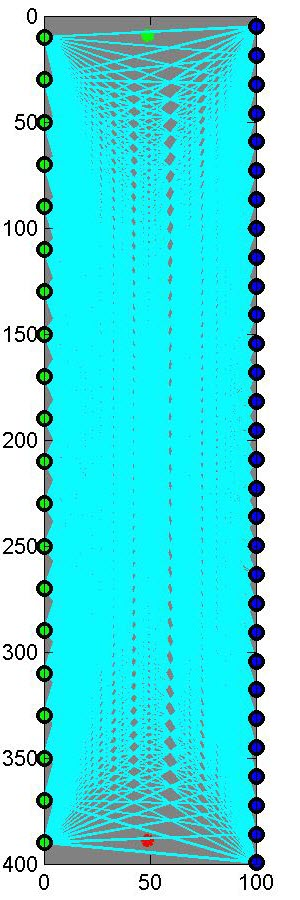
\includegraphics[width=1\iwidth]{figures/initialExperiment}
%			&
%			\includegraphics[width=1\iwidth]{figures/flow}\\			
%			\hline
%		\end{tabular}
%	\end{center}
%\caption{Initial experiment setup. Tomography sources are pictured in green on the left and receivers in blue on. The initial setup covers the entire flow domain with 20 sources and 30 receivers. There is one source of fluid, pumped at a constant rate from the top green point, and a sink at the bottom (red) of the domain. Flow is thus in the downward direction. }
%\label{fig:surveyDesign}
%\end{figure}
\begin{figure}
	\renewcommand{\arraystretch}{1.5}
	\begin{center}
		\iwidth=90mm			
			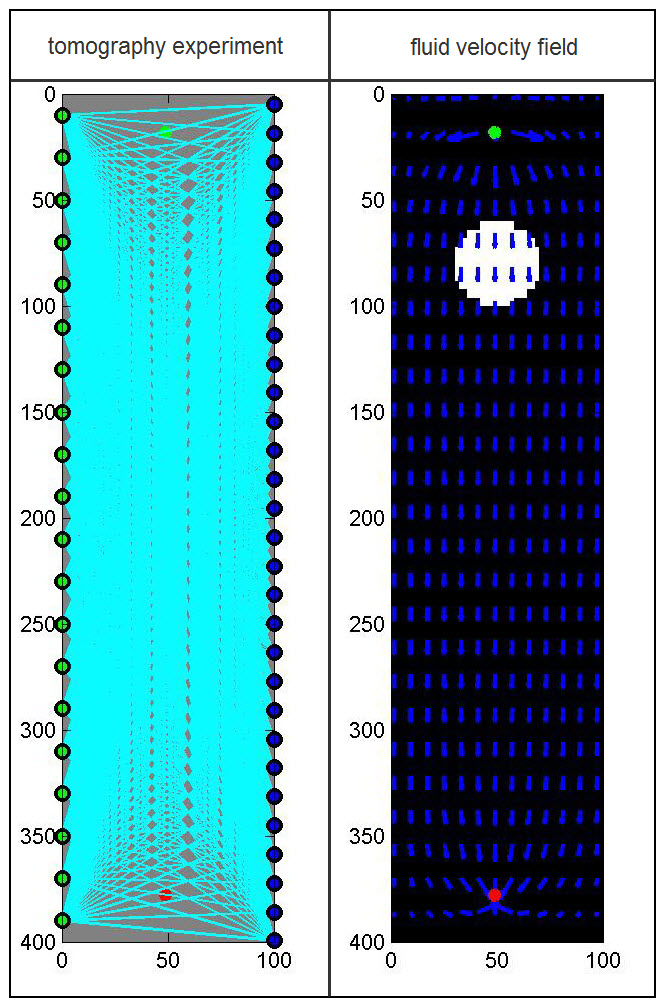
\includegraphics[width=1\iwidth]{figures/initialSetUp}			
	\end{center}
\caption{Initial experiment setup. Tomography sources are pictured in green on the left and receivers in blue on the right. The initial setup covers the entire flow domain with 20 sources and 30 receivers. There is one source of fluid, pumped at a constant rate from the top green point, and a sink at the bottom (red) of the domain. Flow is in the downward direction. }
\label{fig:surveyDesign}
\end{figure}
\subsection{Regularization}

Two different inversions were carried out to recover models $\bfm_k$, by apply two different regularization functions.  
First a linear inversion was performed where the operator $\bfL$ was chosen to be a gradient operator,  $\bfL = \GRADh$, to promote smoothness in the recovered models.

Second, a non-linear inversion was performed with smoothed total variation (TV) as the  regularization~\cite{Ascher2006}.
 The total variation regularization promotes discontinuous boundaries, or sharp edges. This is particularly valid for our experiment since we have chosen advection without a diffusion term to transport a concentration of tracer. The tracer model is  concentrated in the circle and zero everywhere else. In this ideal case there should be no diffusion of the tracer, and thus the boundaries should remain sharp as it is advected along in the fluid velocity field.

In continuous space, smoothed total variation is described by the following relation,
\begin{equation}
		R(m) = \alpha \int  \phi(|\grad m|) \ d\vx.
\end{equation} 
where the convex function $\phi(c) = \sqrt{c^2 + \epsilon}$, is an approximation to the $\ell_1$ norm. 

A standard discrete 
approximation for the smoothed total variation regularization found in ~\cite{Ascher2006} is, 
\begin{equation}
\label{regsd}
R(\bfm) = \alpha h^2 \bfe^{\top} \sqrt{ \bfA_{f}^{c} \left( (\GRADh\ \bfm) \odot (\GRADh\ \bfm) \right)  + \epsilon},
\end{equation}
where the  gradient operator, $\GRADh$,   maps from cell centers to cell faces, and the averaging matrix $\bfA_{f}^{c}$ maps from faces to cell centers. 

Although we have formulated the optimal design based on a linear estimation of $\bfm_k$, it is not unreasonable to estimate $\bfm_k$  with a non-linear regularization, provided that this will contribute to recovering the best estimates of $\bfm_k$. As can be seen in figure \ref{fig:erro1} below, the overall relative model error for estimates recovered with the total variation regularization is significantly lower than that of the models estimated using the linear regularization. Thus the estimates obtained using the TV regularization are more accurate with respect to the true model for this particular problem. 
Since the monitor function has a very large impact on the optimal design, it is desirable to get the best possible estimate of $\bfm_k$. 
%
\begin{figure}
\begin{center}
\iwidth=180mm
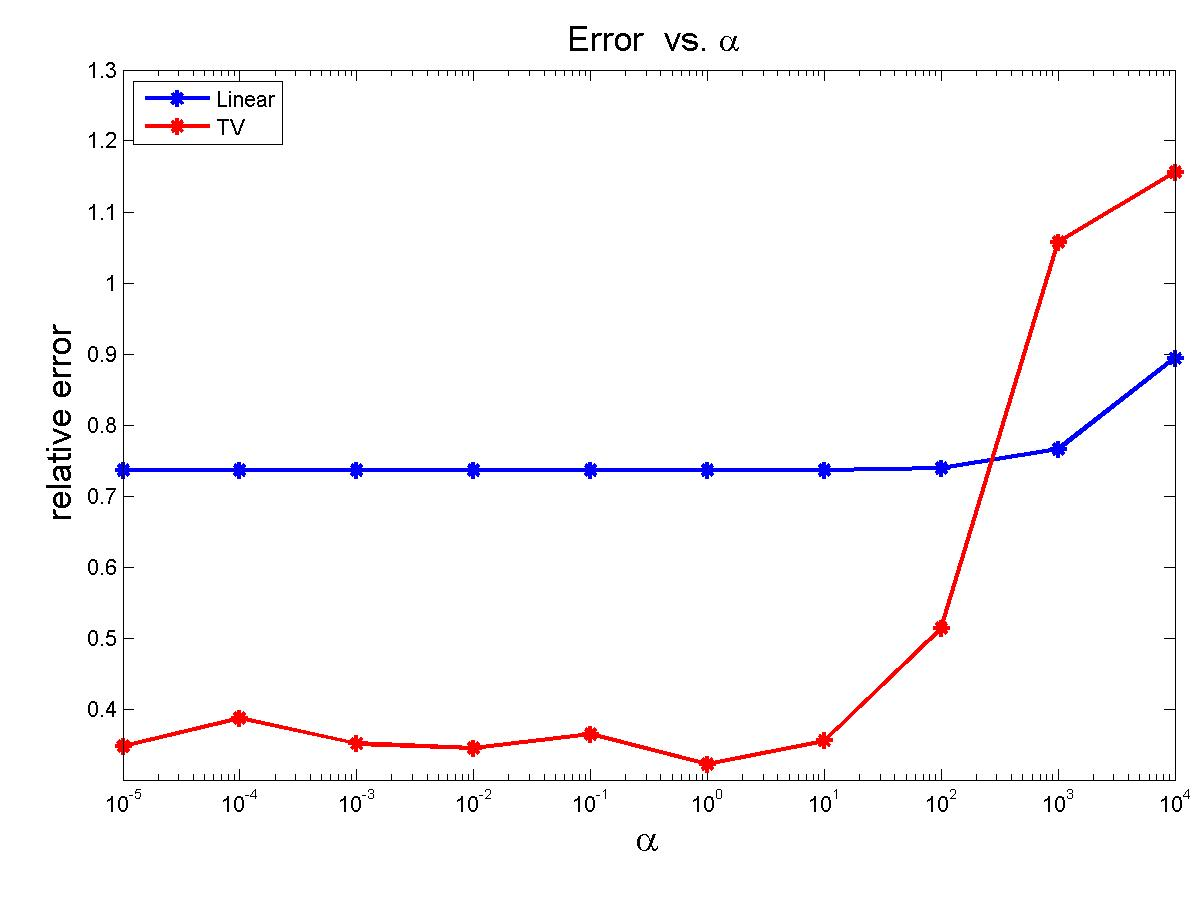
\includegraphics[width=.75\iwidth]{figures/newFigs/exp2-error1}
\end{center}
\caption{Plot of the relative error ($\|\bfm_1^{true}-\bfmhat_1\|/(    \|\bfm^{true}_1\|)$) versus the regularization parameter $\alpha$ for both the linear regularization and smoothed total variation. }
	\label{fig:erro1}
\end{figure} 

In all cases, the regularization parameter had the value $\alpha_k = 100$. This value was chosen following a cooling strategy which starts with a large value for $\alpha$. Alpha is then decreased incrementally after each inversion, until the data misfit is approximately equal to noise.



\subsection{Monitor function}

To design only for the tracer motion, we define delta as $\bfdelta = |\bfm_{k} -\bfm_{\text{background}}|$. Because  neither the estimated model nor the background model are perfect, we  chose a threshold value $s$ to remove unwanted or erroneous information from delta 
%and defined the monitor function tau as a characteristic functions
%as follows,
%\begin{equation*}
%\bftau_{B} =  
%\begin{cases}
%0, & \text{if } \bfdelta \leq s\\
%1, & \text{if } \bfdelta > s
%\end{cases}
%\end{equation*}
where the background model $\bfm_{\text{background}} $, is the model used to compute the velocity field in equation \eqref{eq:flowu}.

\section{Design results: Noiseless dynamics}
\label{sec:Results}
For the noiseless case, data were simulated by marching  the initial tracer concentration along in time, for time steps of 25 days and measured by conducting a tomography survey at each time with 4\% Gaussian noise added to each data set. In total 9 experiments were conducted for times $t_0,t_1,...,t_8$. 


The initial design for time point $t_0$ did not include the dynamics. This amounts to  setting $\bftau_0 = 1$ everywhere. The design optimization problem in this case is  identical to the static case and produces an optimal design based only on the physics and information from the linear regularization operator $\bfL$. This is apparent in both the plot of the weights for experiment 1 at time  $t_0$ in figure \ref{fig:weights1} and the image of the rays in figure \ref{fig:results1}, where the design specifies fewer rays that cover the entire domain. 

For each experiment the amse was plotted versus the number of nonzero weights for a set of regularization parameters $\beta$, see figure \ref{fig:weights1} for examples for times $t_0,t_2,t_4$. From these curves, the best set of weights were chosen such that the weights were sparse, but also so the amse was kept reasonably small. 
%\begin{figure}[!h]
%	\renewcommand{\arraystretch}{1.5}
%	\begin{center}
%		\iwidth=90mm
%		\begin{tabular}{|c|c|c|} %{@{}|@{\ }p{3mm}@{}|@{\ }c@{\;}|@{\;}c@{\ }|}
%			\hline		
%			exp & sparsity & weights	\\
%			\hline	
%			$1$
%			&	
%			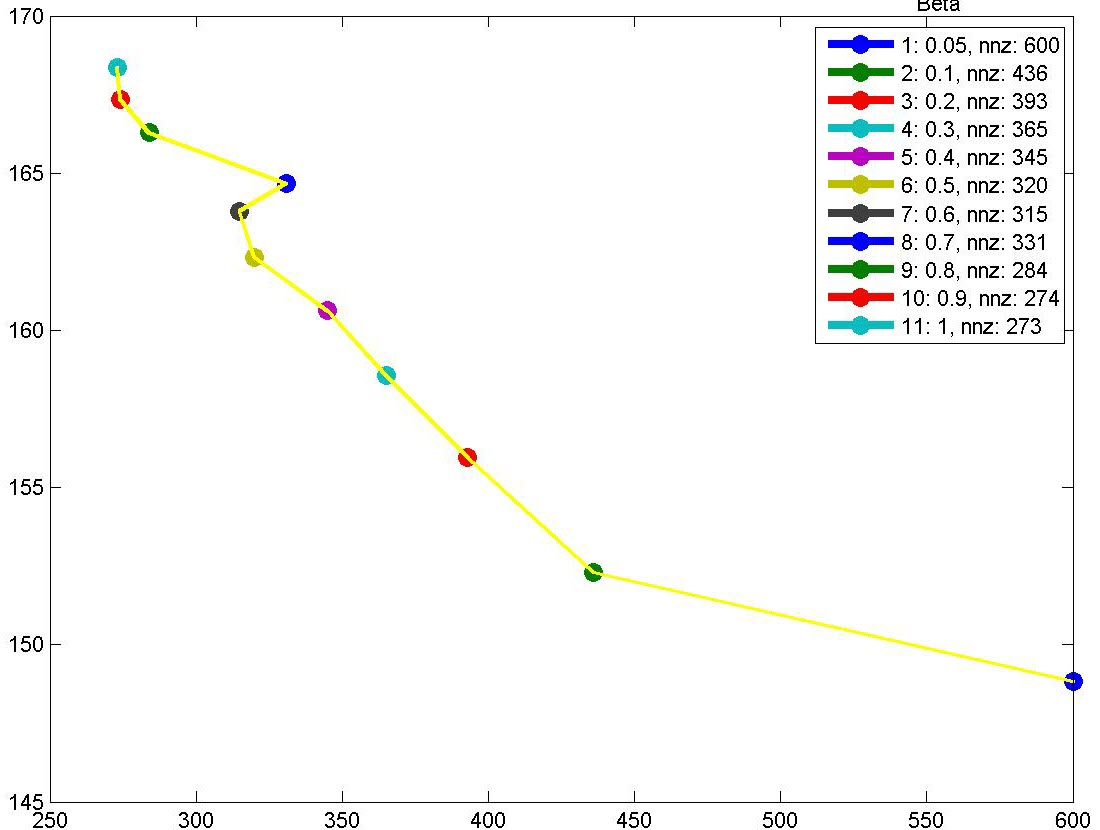
\includegraphics[width=.65\iwidth]{figures/newFigs/exp1paretoWeights}
%			&
%			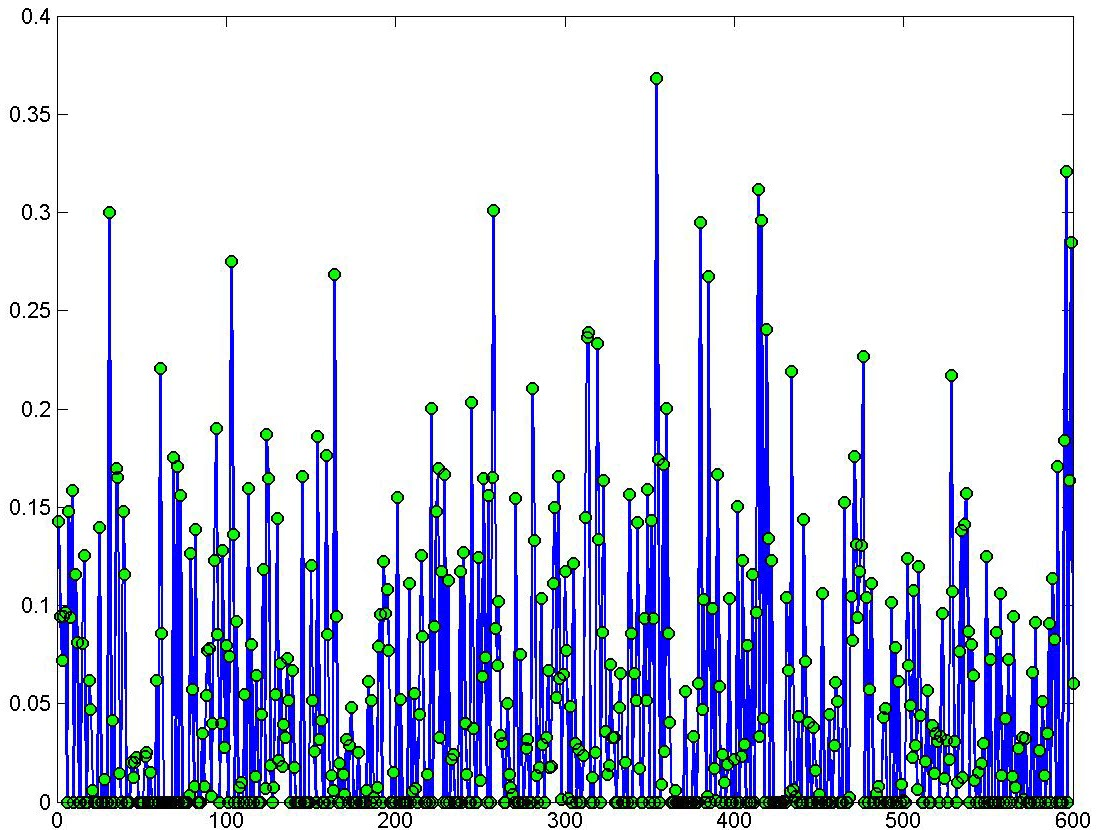
\includegraphics[width=.65\iwidth]{figures/newFigs/exp1Weights}\\
%			\hline
%			$3$
%			&	
%			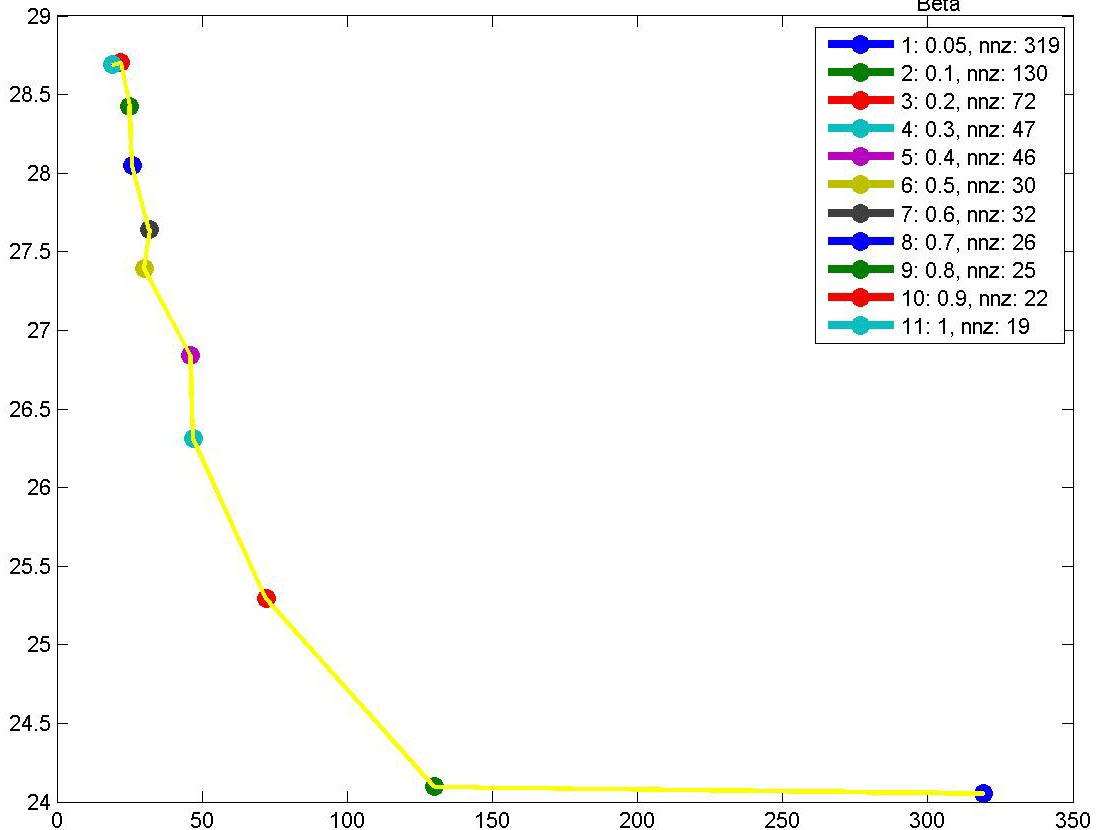
\includegraphics[width=.65\iwidth]{figures/newFigs/exp3paretoWeights}
%			&
%			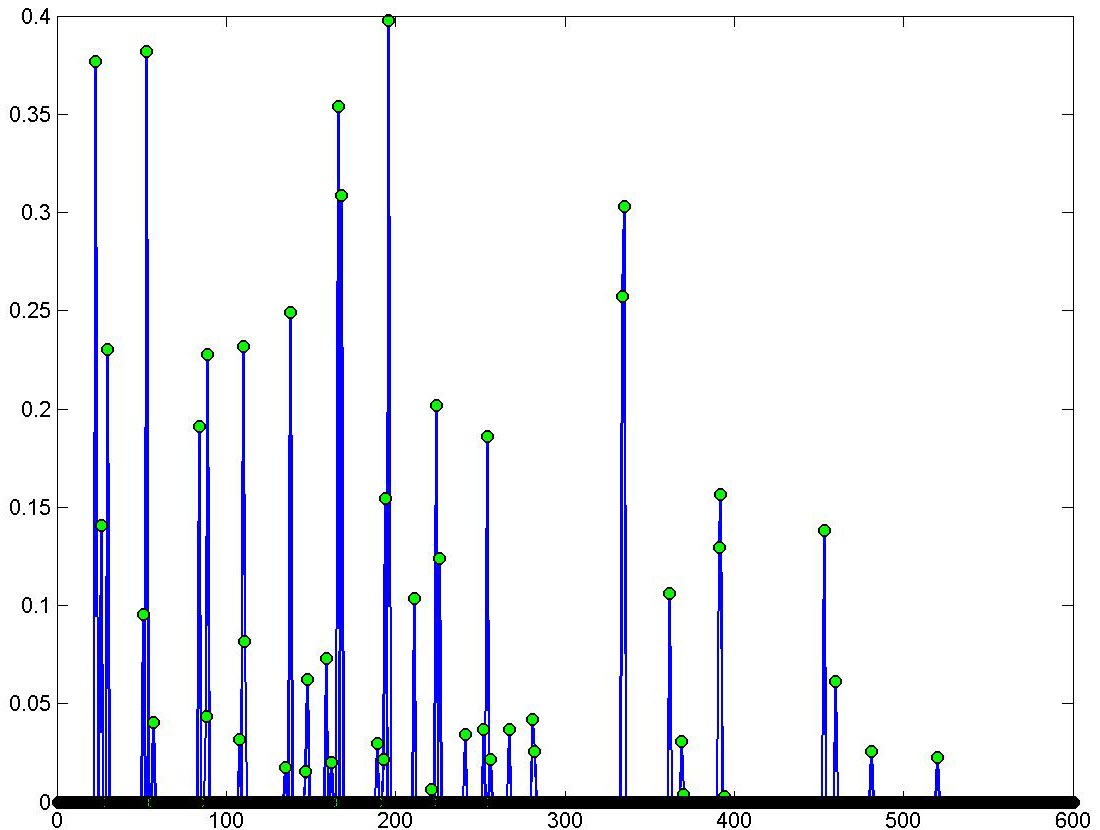
\includegraphics[width=.65\iwidth]{figures/newFigs/exp3Weights}\\
%			\hline
%			$5$
%			&	
%			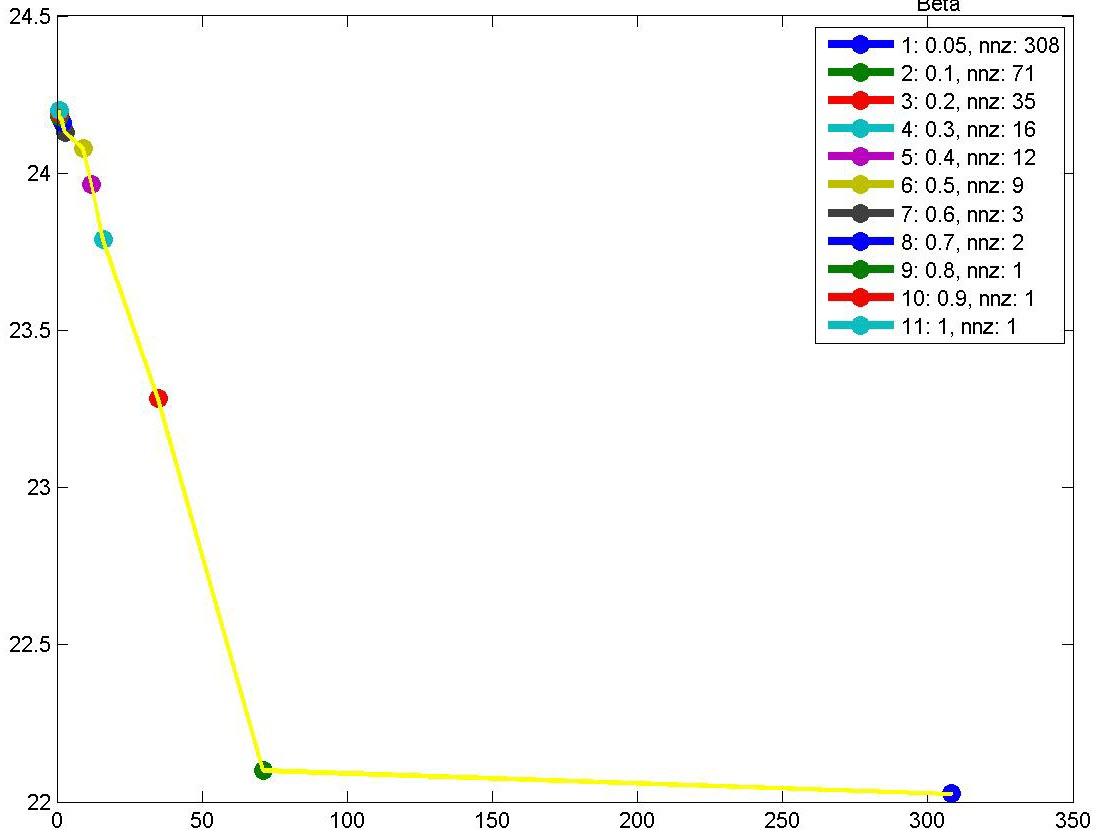
\includegraphics[width=.65\iwidth]{figures/newFigs/exp5paretoWeights}
%			&
%			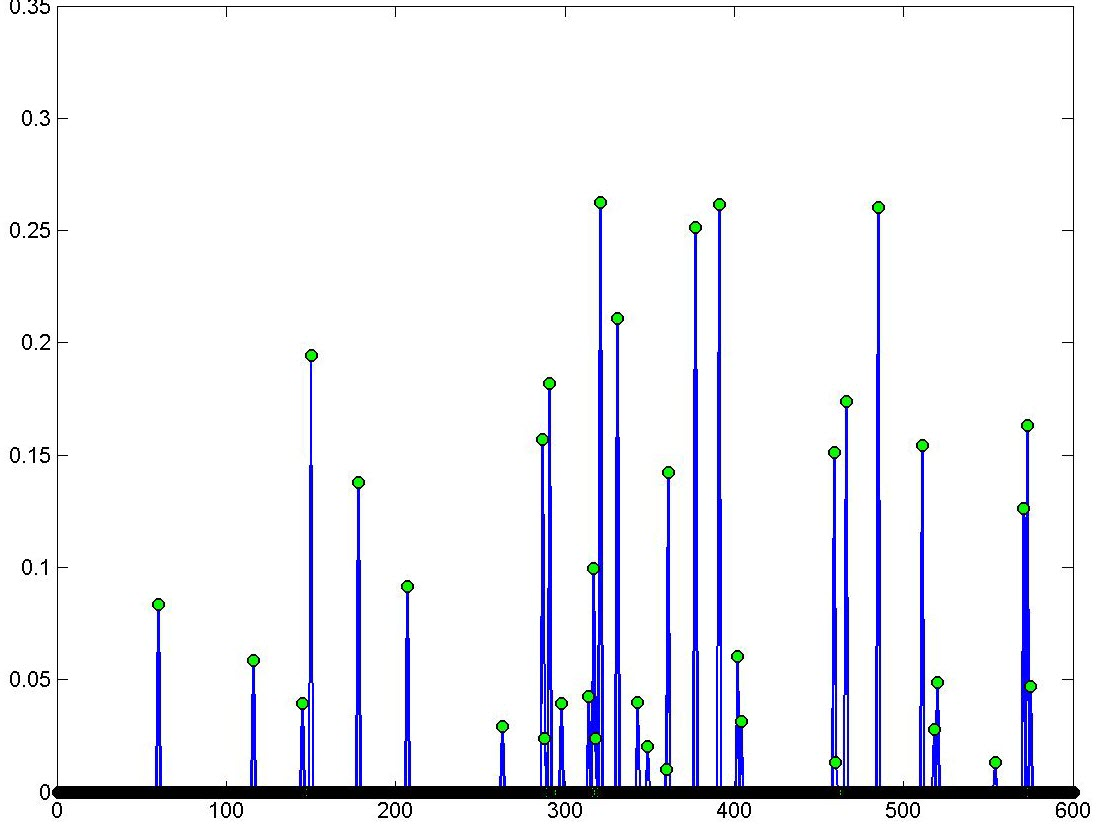
\includegraphics[width=.65\iwidth]{figures/newFigs/exp5Weights}\\			
%			\hline
%		\end{tabular}
%	\end{center}
%	\caption{Noiseless dynamics: Plots of the amse  vs. the number of nonzero weights (left column), and the weights used to conduct the experiment for experiments 1,3,and 5, at times $t_0,t_2,t_4$.}
%	\label{fig:weights1}
%\end{figure}


\begin{figure}
	\renewcommand{\arraystretch}{1.5}
	\begin{center}
		\iwidth=130mm
					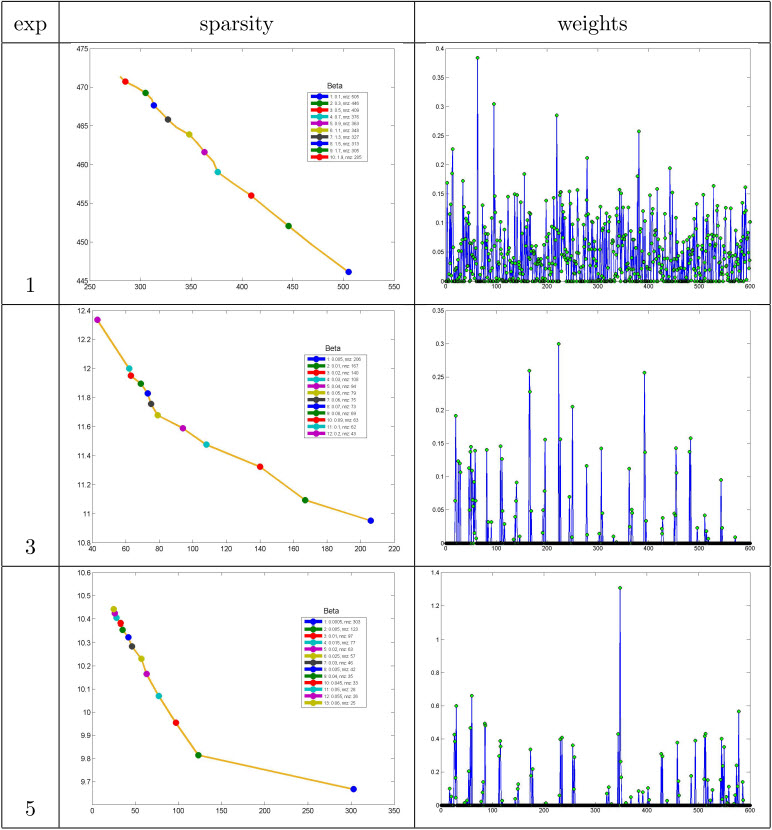
\includegraphics[width=1\iwidth]{figures/risk2}
	\end{center}
	\caption{Noiseless dynamics: Plots of the amse  vs. the number of nonzero weights (left column), and the weights used to conduct the experiment for experiments 1, 3, and 5, at times $t_0,\; t_2,\; t_4$.}
	\label{fig:weights1}
\end{figure}
After a set of weights were chosen, both $\bfm_0$ and the current model $\bfm_k$ were reconstructed from the reduced set of data $\bfd_k$. The values of $\bfd$ which contribute to the reduced data set correspond to the non-zero weights of $\bfw_k$. The total number of data required to image the models is significantly reduced. In most cases the number of data are on average  40 of a possible 600.
  In figure \ref{fig:results1} the rays corresponding to $\bfd_k$ used to estimate the current models are pictured in blue over an image of the model. Note that the rays tend to follow the target as it moves through the domain and pass through the tracer.
There are some spurious rays that do not pass through the tracer which are included in the optimal design. However, since the design depends on the monitor function  $\bftau(\bfmhat_0)$, and the reconstructions of $\bfmhat_0$ are never exact,  these spurious rays are expected. 

It is also apparent that the number of spurious rays increases further in time even though estimates of $\bfm_0$ improve as more data are collected. In particular, at time $t_6$ it appears that the design algorithm has a harder time generating a design that captures the target well. There are many more rays which do not pass through the target. This is partially due to the increasing number of multiplications by the transport matrix $\bfT$ as time progresses, compounding errors, but also the loss of mass as the tracer exits the domain out of the sink. However, the designs still provide enough information to recover models which indicate the location of the tracer.  

The reconstructions of $\bfm_k$ with smoothed total variation as the regularization are much closer to the true models, even when the optimal design was computed for the linear regularization model estimation problem. Again, this is to be expected since we have chosen a model with discontinuous edges, and are transporting the target only by advection. 
\begin{figure}
	\begin{center}
	\iwidth=170mm
	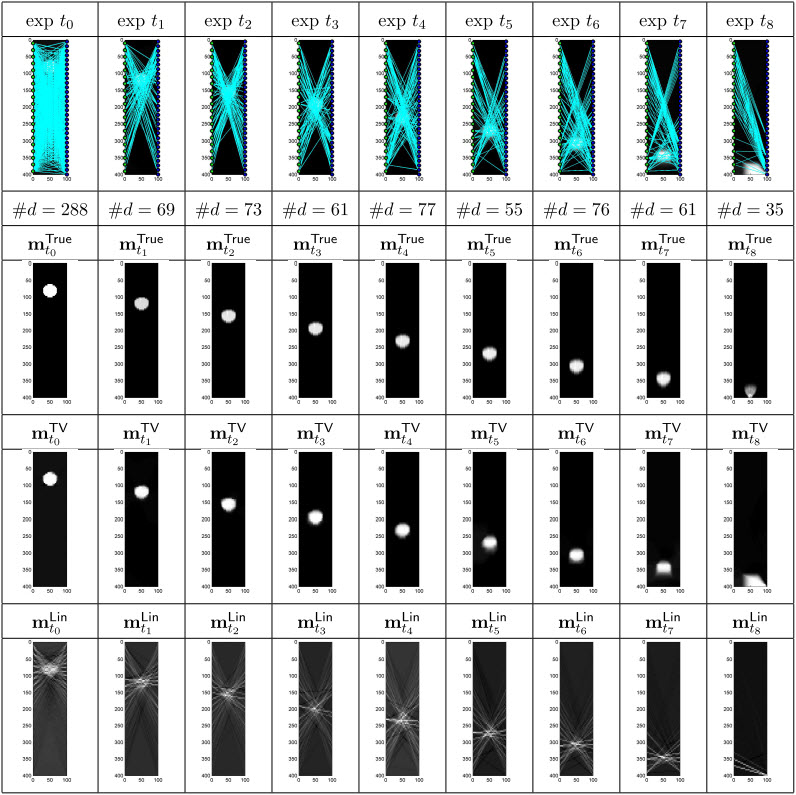
\includegraphics[width = 1\iwidth]{figures/noiselessFigs/noiselessResults}
	\end{center}
	\caption{Noiseless dynamics: Optimal designs and recovered models for 9 	experiments. The top row shows the rays and the recovered model, with 		the number of rays (\#d = 350) given below, followed by the true 			models, the models recovered using total variation, and finally the 		models recovered using the linear gradient regularization.}
	\label{fig:results1}
\end{figure}

%
%\begin{figure}[!h]
%	\renewcommand{\arraystretch}{1.5}
%	\begin{center}
%		\iwidth=13mm
%		\begin{tabular}{|c|c|c|c|c|c|c|c|c|}
%			\hline		
%			 exp $t_0$ & exp $t_1$ & exp $t_2$& exp $t_3$& exp $t_4$& exp $t_5$& exp $t_6$ & exp $t_7$ & exp $t_8$\\
%			\hline		
%			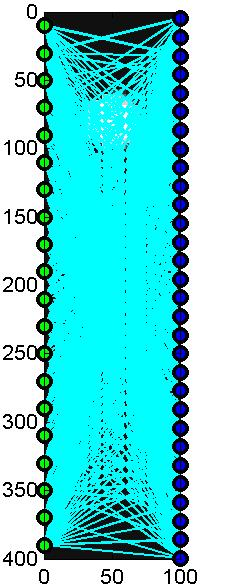
\includegraphics[width=.9\iwidth]{figures/noiselessFigs/resultsExp-1-designs}
%			&
%			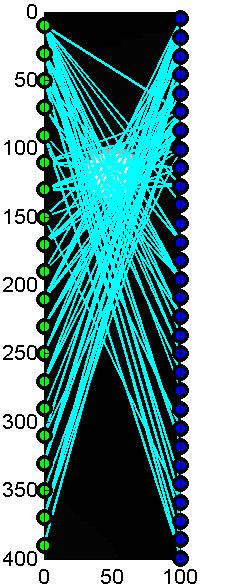
\includegraphics[width=.9\iwidth]{figures/noiselessFigs/resultsExp-2-designs}
%			&
%			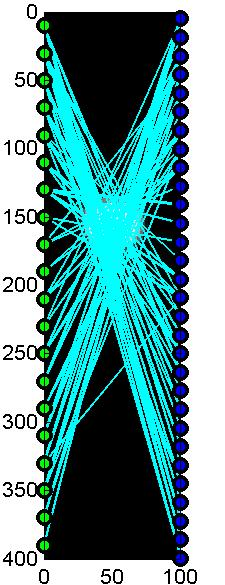
\includegraphics[width=.9\iwidth]{figures/noiselessFigs/resultsExp-3-designs}
%			&
%			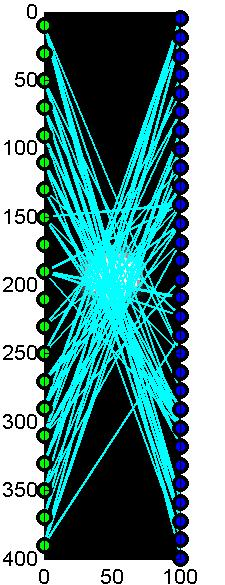
\includegraphics[width=.9\iwidth]{figures/noiselessFigs/resultsExp-4-designs}
%			&
%			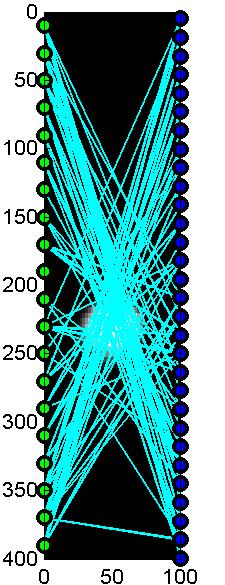
\includegraphics[width=.9\iwidth]{figures/noiselessFigs/resultsExp-5-designs}
%			&
%			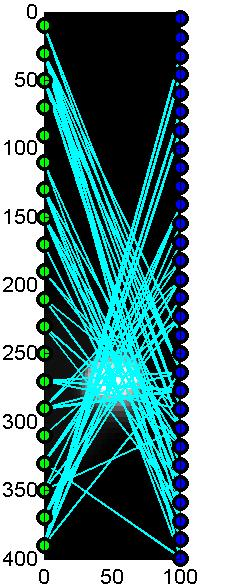
\includegraphics[width=.9\iwidth]{figures/noiselessFigs/resultsExp-6-designs}
%			&
%			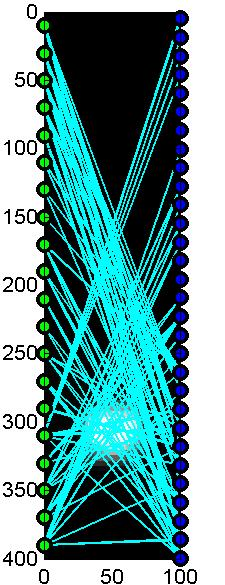
\includegraphics[width=.9\iwidth]{figures/noiselessFigs/resultsExp-7-designs}
%			&
%			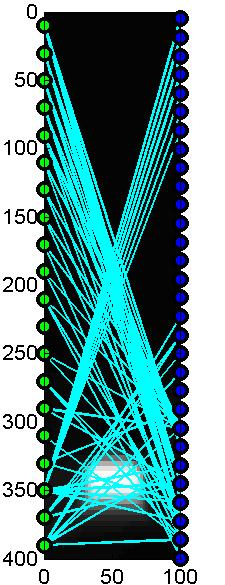
\includegraphics[width=.9\iwidth]{figures/noiselessFigs/resultsExp-8-designs}
%			&
%			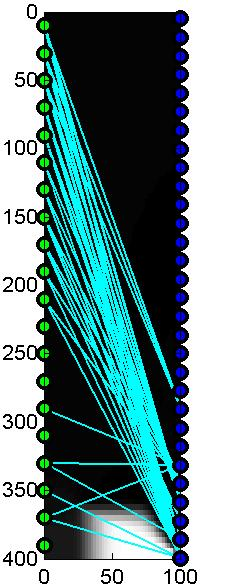
\includegraphics[width=.9\iwidth]{figures/noiselessFigs/resultsExp-9-designs}			
%			\\
%			\hline
%			$\#d=288$& $\#d=69$& $\#d=73$& $\#d= 61$& $\#d=77$& $\#d=55$& $\#d=76$& $\#d=61$& $\# d=35$\\
%			\hline	
%			 $\bfm^{\sf True}_{t_0}$& $\bfm^{\sf True}_{t_1}$&$\bfm^{\sf True}_{t_2}$& $\bfm^{\sf True}_{t_3}$&$\bfm^{\sf True}_{t_4}$& $\bfm^{\sf True}_{t_5}$ &$\bfm^{\sf True}_{t_6}$&$\bfm^{\sf True}_{t_7}$& $\bfm^{\sf True}_{t_8}$ 
%			 \\
%			\hline	
%			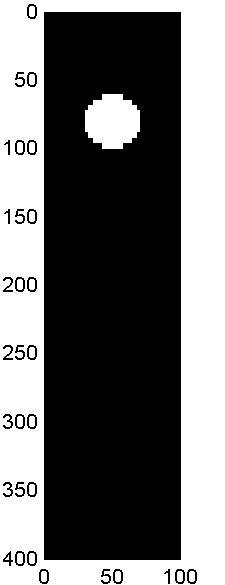
\includegraphics[width=.9\iwidth]{figures/noiselessFigs/resultsExp-1-mtrue}
%			&
%			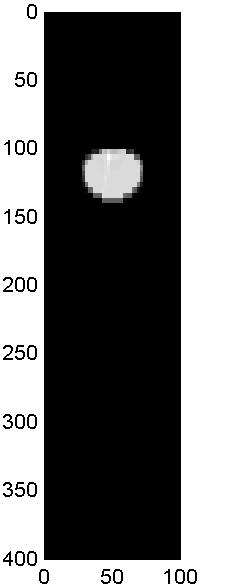
\includegraphics[width=.9\iwidth]{figures/noiselessFigs/resultsExp-2-mtrue}
%			&
%			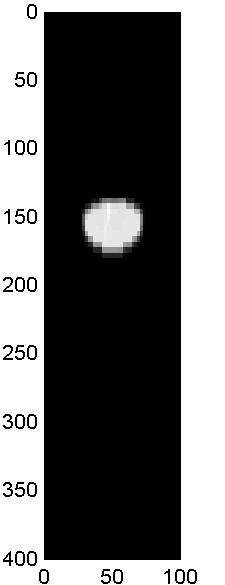
\includegraphics[width=.9\iwidth]{figures/noiselessFigs/resultsExp-3-mtrue}
%			&
%			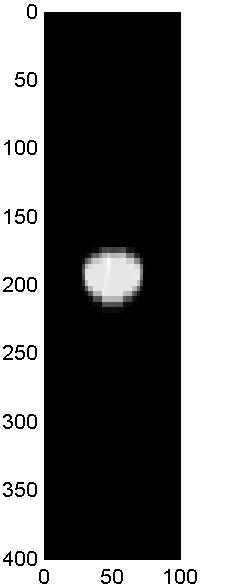
\includegraphics[width=.9\iwidth]{figures/noiselessFigs/resultsExp-4-mtrue}
%			&
%			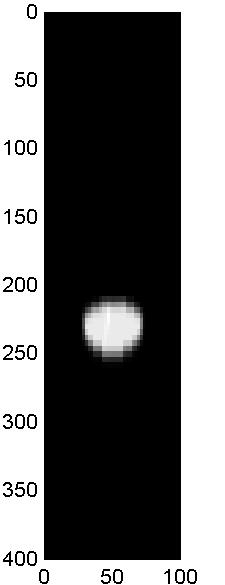
\includegraphics[width=.9\iwidth]{figures/noiselessFigs/resultsExp-5-mtrue}
%			&
%			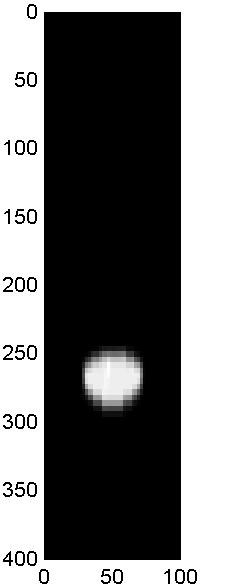
\includegraphics[width=.9\iwidth]{figures/noiselessFigs/resultsExp-6-mtrue}
%			&
%			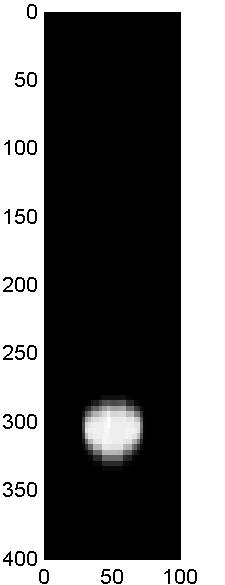
\includegraphics[width=.9\iwidth]{figures/noiselessFigs/resultsExp-7-mtrue}
%			&
%			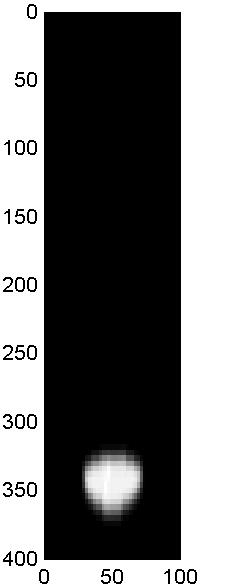
\includegraphics[width=.9\iwidth]{figures/noiselessFigs/resultsExp-8-mtrue}
%			&
%			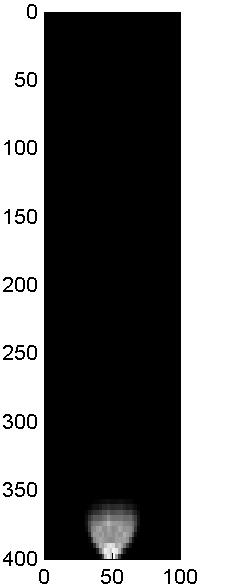
\includegraphics[width=.9\iwidth]{figures/noiselessFigs/resultsExp-9-mtrue}
%			\\
%			\hline
%			 $\bfm^{\sf TV}_{t_0}$& $\bfm^{\sf TV}_{t_1}$&$\bfm^{\sf TV}_{t_2}$& $\bfm^{\sf TV}_{t_3}$&$\bfm^{\sf TV}_{t_4}$& $\bfm^{\sf TV}_{t_5}$ &$\bfm^{\sf TV}_{t_6}$&$\bfm^{\sf TV}_{t_7}$& $\bfm^{\sf TV}_{t_8}$ \\
%			\hline	
%			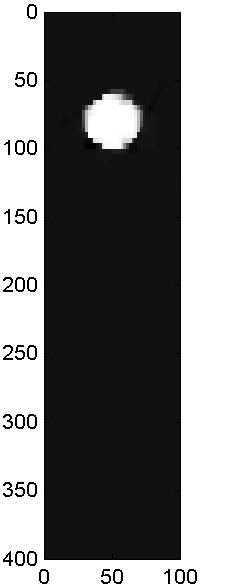
\includegraphics[width=.9\iwidth]{figures/noiselessFigs/resultsExp-1-mkTV}
%			&
%			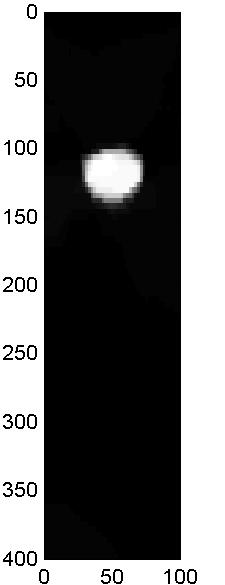
\includegraphics[width=.9\iwidth]{figures/noiselessFigs/resultsExp-2-mkTV}
%			&
%			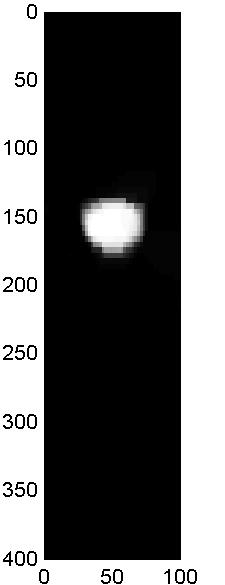
\includegraphics[width=.9\iwidth]{figures/noiselessFigs/resultsExp-3-mkTV}
%			&
%			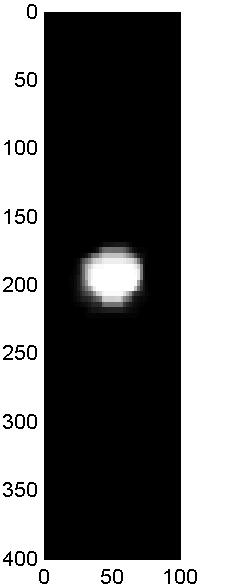
\includegraphics[width=.9\iwidth]{figures/noiselessFigs/resultsExp-4-mkTV}
%			&
%			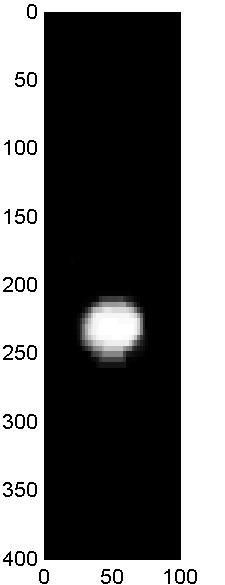
\includegraphics[width=.9\iwidth]{figures/noiselessFigs/resultsExp-5-mkTV}
%			&
%			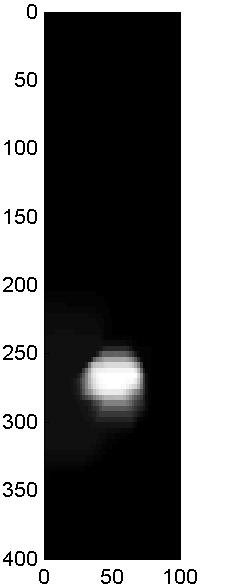
\includegraphics[width=.9\iwidth]{figures/noiselessFigs/resultsExp-6-mkTV}
%			&
%			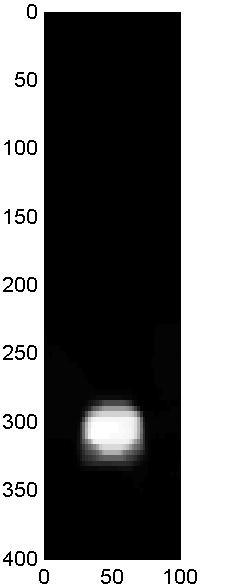
\includegraphics[width=.9\iwidth]{figures/noiselessFigs/resultsExp-7-mkTV}
%			&
%			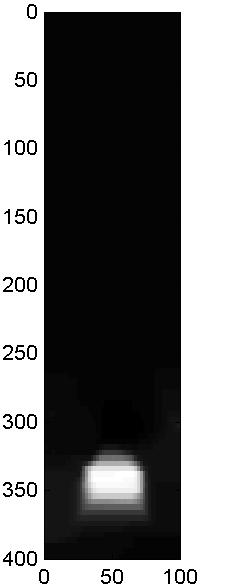
\includegraphics[width=.9\iwidth]{figures/noiselessFigs/resultsExp-8-mkTV}
%			&
%			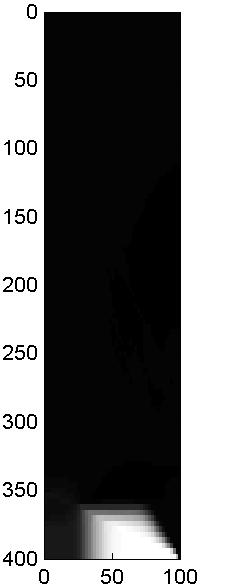
\includegraphics[width=.9\iwidth]{figures/noiselessFigs/resultsExp-9-mkTV}
%			\\
%			\hline	
%			 $\bfm^{\sf Lin}_{t_0}$& $\bfm^{\sf Lin}_{t_1}$&$\bfm^{\sf Lin}_{t_2}$& $\bfm^{\sf Lin}_{t_3}$&$\bfm^{\sf Lin}_{t_4}$& $\bfm^{\sf Lin}_{t_5}$ &$\bfm^{\sf Lin}_{t_6}$&$\bfm^{\sf Lin}_{t_7}$& $\bfm^{\sf Lin}_{t_8}$ \\
%			\hline	
%			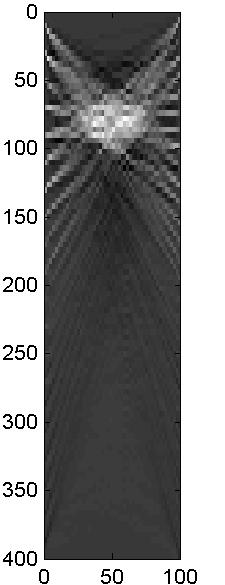
\includegraphics[width=.9\iwidth]{figures/noiselessFigs/resultsExp-1-mk}
%			&
%			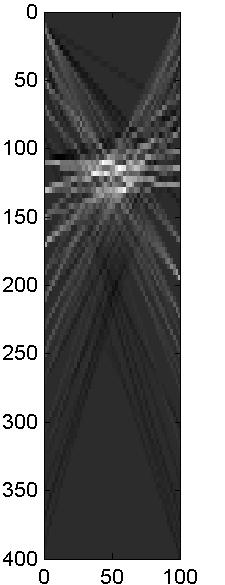
\includegraphics[width=.9\iwidth]{figures/noiselessFigs/resultsExp-2-mk}
%			&
%			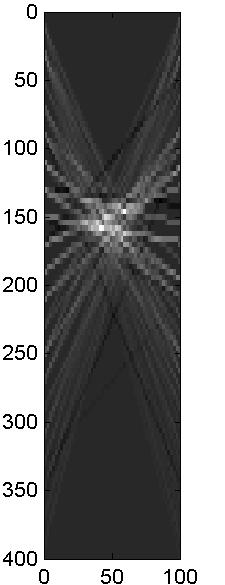
\includegraphics[width=.9\iwidth]{figures/noiselessFigs/resultsExp-3-mk}
%			&
%			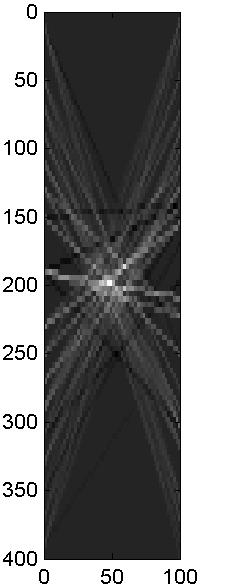
\includegraphics[width=.9\iwidth]{figures/noiselessFigs/resultsExp-4-mk}
%			&
%			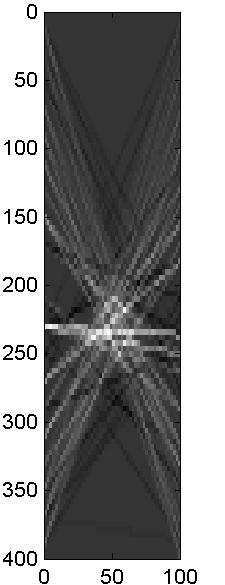
\includegraphics[width=.9\iwidth]{figures/noiselessFigs/resultsExp-5-mk}
%			&
%			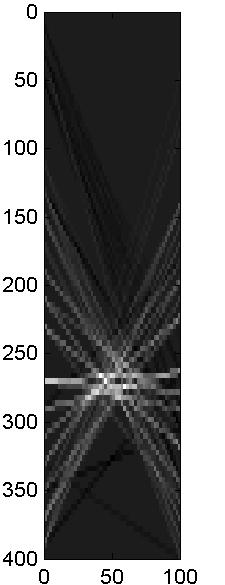
\includegraphics[width=.9\iwidth]{figures/noiselessFigs/resultsExp-6-mk}
%			&
%			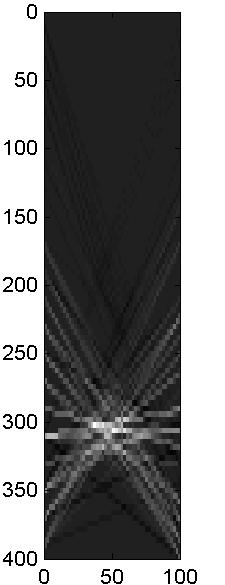
\includegraphics[width=.9\iwidth]{figures/noiselessFigs/resultsExp-7-mk}
%			&
%			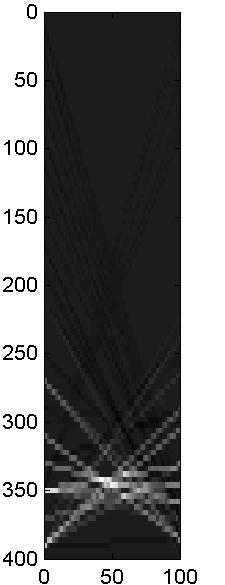
\includegraphics[width=.9\iwidth]{figures/noiselessFigs/resultsExp-8-mk}
%			&
%			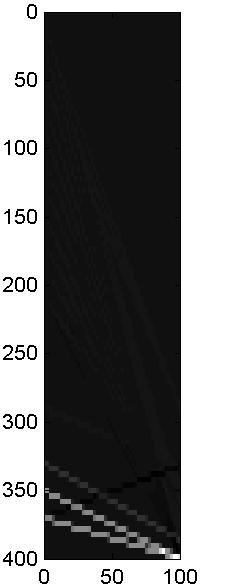
\includegraphics[width=.9\iwidth]{figures/noiselessFigs/resultsExp-9-mk}		
%			\\			
%			\hline
%		\end{tabular}
%	\end{center}
%	\caption{Noiseless dynamics: Optimal designs and recovered models for 9 experiments. The top row shows the rays and the recovered model, with the number of rays (\#d = 350) given below, followed by the true models, the models recovered using total variation, and finally the models recovered using the linear gradient regularization.}
%	\label{fig:results1}
%\end{figure}


\section{Results: Noisy  dynamics}
\label{sec: Example2}
For the first experiment $\bfw_0$, the initial naive experiment computed in the noiseless example was used in the subsequent design estimations. Each model was reconstructed at each time step after using the reduced data sets determined by the optimal design. Models were reconstructed using the non-linear smoothed total variation regularization, and also with the linear regularization. 
The covariance matrices $\bfQ_k$ were assigned a scalar value for the variance for each time step to represent iid noise in the dynamics, such that $\bfQ_k = \sigma_k \bfI$. We assigned a constant $\sigma_k = \pm 0.2$ for all experiments. 

The results are pictured in figure \ref{fig:results2}, below. It is apparent that adapted A-optimal designs were again able to track the motion of the tracer with a significantly reduced set of measurements. The recoveries for $\bfm_k$ using the linear regularization term approximate the true models to a better extent that those of the noiseless formulation. However, those recovered with the smoothed TV regularization were again used in the monitor function. 
\begin{figure}
	\begin{center}
	\iwidth=170mm
	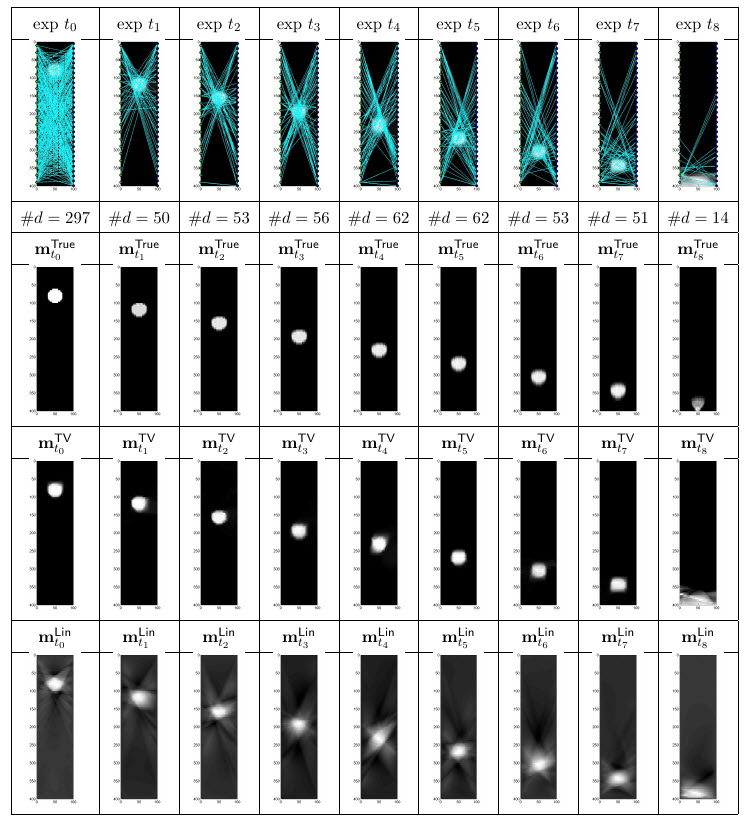
\includegraphics[width = 1\iwidth]{figures/newFigs/resultsAll2-new}
	\end{center}
	\caption{Noisey dynamics: Optimal designs and recovered models for 9 experiments. The top row shows the rays and the recovered model, with the number of rays (ex. \#d = 297) given below. The second row pictures true models, the third shows the  models recovered using total variation, and finally the bottom shows models recovered using the linear gradient regularization.}
	\label{fig:results2}
\end{figure}
%
%\begin{figure}[!h]
%	\renewcommand{\arraystretch}{1.5}
%	\begin{center}
%		\iwidth=13mm
%		\begin{tabular}{|c|c|c|c|c|c|c|c|c|}
%			\hline		
%			 exp $t_0$ & exp $t_1$ & exp $t_2$& exp $t_3$& exp $t_4$& exp $t_5$& exp $t_6$ & exp $t_7$ & exp $t_8$\\
%			\hline		
%			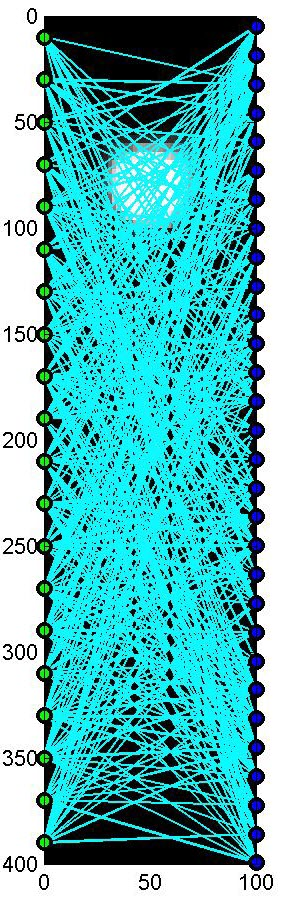
\includegraphics[width=.9\iwidth]{figures/newFigs/noisy/resultsExp-1-designs}
%			&
%			\includegraphics[width=.9\iwidth]{figures/newFigs/noisy/resultsExp-2-designs}
%			&
%			\includegraphics[width=.9\iwidth]{figures/newFigs/noisy/resultsExp-3-designs}
%			&
%			\includegraphics[width=.9\iwidth]{figures/newFigs/noisy/resultsExp-4-designs}
%			&
%			\includegraphics[width=.9\iwidth]{figures/newFigs/noisy/resultsExp-5-designs}
%			&
%			\includegraphics[width=.9\iwidth]{figures/newFigs/noisy/resultsExp-6-designs}
%			&
%			\includegraphics[width=.9\iwidth]{figures/newFigs/noisy/resultsExp-7-designs}
%			&
%			\includegraphics[width=.9\iwidth]{figures/newFigs/noisy/resultsExp-8-designs}
%			&
%			\includegraphics[width=.9\iwidth]{figures/newFigs/noisy/resultsExp-9-designs}			
%			\\
%			\hline
%			$\#d=297$& $\#d=50$& $\#d=53$& $\#d= 56$& $\#d=62$& $\#d=62$& $\#d=53$& $\#d=51$& $\# d=14$\\
%			\hline	
%			 $\bfm^{\sf True}_{t_0}$& $\bfm^{\sf True}_{t_1}$&$\bfm^{\sf True}_{t_2}$& $\bfm^{\sf True}_{t_3}$&$\bfm^{\sf True}_{t_4}$& $\bfm^{\sf True}_{t_5}$ &$\bfm^{\sf True}_{t_6}$&$\bfm^{\sf True}_{t_7}$& $\bfm^{\sf True}_{t_8}$ 
%			 \\
%			\hline	
%			\includegraphics[width=.9\iwidth]{figures/newFigs/noisy/resultsExp-1-mtrue}
%			&
%			\includegraphics[width=.9\iwidth]{figures/newFigs/noisy/resultsExp-2-mtrue}
%			&
%			\includegraphics[width=.9\iwidth]{figures/newFigs/noisy/resultsExp-3-mtrue}
%			&
%			\includegraphics[width=.9\iwidth]{figures/newFigs/noisy/resultsExp-4-mtrue}
%			&
%			\includegraphics[width=.9\iwidth]{figures/newFigs/noisy/resultsExp-5-mtrue}
%			&
%			\includegraphics[width=.9\iwidth]{figures/newFigs/noisy/resultsExp-6-mtrue}
%			&
%			\includegraphics[width=.9\iwidth]{figures/newFigs/noisy/resultsExp-7-mtrue}
%			&
%			\includegraphics[width=.9\iwidth]{figures/newFigs/noisy/resultsExp-8-mtrue}
%			&
%			\includegraphics[width=.9\iwidth]{figures/newFigs/noisy/resultsExp-9-mtrue}
%			\\
%			\hline
%			 $\bfm^{\sf TV}_{t_0}$& $\bfm^{\sf TV}_{t_1}$&$\bfm^{\sf TV}_{t_2}$& $\bfm^{\sf TV}_{t_3}$&$\bfm^{\sf TV}_{t_4}$& $\bfm^{\sf TV}_{t_5}$ &$\bfm^{\sf TV}_{t_6}$&$\bfm^{\sf TV}_{t_7}$& $\bfm^{\sf TV}_{t_8}$ \\
%			\hline	
%			\includegraphics[width=.9\iwidth]{figures/newFigs/noisy/resultsExp-1-mkTV}
%			&
%			\includegraphics[width=.9\iwidth]{figures/newFigs/noisy/resultsExp-2-mkTV}
%			&
%			\includegraphics[width=.9\iwidth]{figures/newFigs/noisy/resultsExp-3-mkTV}
%			&
%			\includegraphics[width=.9\iwidth]{figures/newFigs/noisy/resultsExp-4-mkTV}
%			&
%			\includegraphics[width=.9\iwidth]{figures/newFigs/noisy/resultsExp-5-mkTV}
%			&
%			\includegraphics[width=.9\iwidth]{figures/newFigs/noisy/resultsExp-6-mkTV}
%			&
%			\includegraphics[width=.9\iwidth]{figures/newFigs/noisy/resultsExp-7-mkTV}
%			&
%			\includegraphics[width=.9\iwidth]{figures/newFigs/noisy/resultsExp-8-mkTV}
%			&
%			\includegraphics[width=.9\iwidth]{figures/newFigs/noisy/resultsExp-9-mkTV}
%			\\
%			\hline	
%			 $\bfm^{\sf Lin}_{t_0}$& $\bfm^{\sf Lin}_{t_1}$&$\bfm^{\sf Lin}_{t_2}$& $\bfm^{\sf Lin}_{t_3}$&$\bfm^{\sf Lin}_{t_4}$& $\bfm^{\sf Lin}_{t_5}$ &$\bfm^{\sf Lin}_{t_6}$&$\bfm^{\sf Lin}_{t_7}$& $\bfm^{\sf Lin}_{t_8}$ \\
%			\hline	
%			\includegraphics[width=.9\iwidth]{figures/newFigs/noisy/resultsExp-1-mk}
%			&
%			\includegraphics[width=.9\iwidth]{figures/newFigs/noisy/resultsExp-2-mk}
%			&
%			\includegraphics[width=.9\iwidth]{figures/newFigs/noisy/resultsExp-3-mk}
%			&
%			\includegraphics[width=.9\iwidth]{figures/newFigs/noisy/resultsExp-4-mk}
%			&
%			\includegraphics[width=.9\iwidth]{figures/newFigs/noisy/resultsExp-5-mk}
%			&
%			\includegraphics[width=.9\iwidth]{figures/newFigs/noisy/resultsExp-6-mk}
%			&
%			\includegraphics[width=.9\iwidth]{figures/newFigs/noisy/resultsExp-7-mk}
%			&
%			\includegraphics[width=.9\iwidth]{figures/newFigs/noisy/resultsExp-8-mk}
%			&
%			\includegraphics[width=.9\iwidth]{figures/newFigs/noisy/resultsExp-9-mk}		
%			\\			
%			\hline
%		\end{tabular}
%	\end{center}
%	\caption{Noisey dynamics: Optimal designs and recovered models for 9 experiments. The top row shows the rays and the recovered model, with the number of rays (ex. \#d = 297) given below. The second row pictures true models, the third shows the  models recovered using total variation, and finally the bottom shows models recovered using the linear gradient regularization.}
%	\label{fig:results2}
%\end{figure}


\section{Concluding remarks}
In this paper we have presented a new method for the design of experiments for dynamical systems which tracks the motion of specific areas of the model by incorporating historic data. 
The motivation for not simply applying static optimal design methods to the dynamic problem is that the mean squared error of the current estimated model never contains information from previous data.
To this end, the design optimization problem ``knows'' nothing about the changes in  the model due to the dynamics and thus designs only reflect information from the physics and the regularization of the ill-posed model estimation problem.  

Our adaptive optimal experimental design approach is based on the introduction of a monitor function to scale the  mean squared error (amse) of an estimator whose motion is governed by a dynamical system, according to historic data. 
To determine a design for a future experiment, we minimize the amse  with the added constraint that the design is sparse. We consider two model estimation problems whose construction depends on the characterization of the error in the dynamical system. 
This leads to experimental designs which track the changes in the model with a reduced set of measurements.  
We have tested our methodology for a geophysical imaging inverse problem where the dynamics of the  model parameters are governed by advection in porous media. 

\bigskip

%Some thoughts on future work:
%\begin{itemize}
%\item How to do this for non-linear problems -linearize... approximating the mse...propagating models to generate a training set is an option, but not really anything new or different from the non-linear design ill-posed paper...
%\item What other options for including data? What other statistics? 
%\item 3D would be fun for a more applied problem... advection-diffusion or 2-phase flow with the full waveform seismic survey...
%\end{itemize}
\newpage
\bibliographystyle{plain}
\bibliography{designBib}
%\bibliography{../../../../Biblio/biblio}
\end{document}




%\bigskip
%The adaptive design method is outlined in  algorithm \ref{algo1} below.
%\begin{algorithm}
%\caption{Adaptive Optimal Design: Noiseless dynamics}\label{algo1}
%\begin{algorithmic}[1]
%%1
%\State Given a prior $\bfmhat_{0}$  for $\bfm$, set $\bftau(\bfmhat_0)$
%\Comment{if there is no prior, $\bftau = \bfI$}
%%2
%\For{$k = 1 \text{ to } n$}  
%\Comment{ $n$ time points}
%%3
%\State $\bfw_{k} = {\sf argmin }\;\;\ \phi_k(\bfw_k) + \beta\bfe^{\top}\bfw_k$ \Comment{design using equation \eqref{eq:noiselessPhi}} 
%%4
%\State Given $\bfw_k$ collect data $\bfd_k$
%%
%%5
%\State $\bfmhat_{0,k} ={\sf argmin } \;\; \hf  \sum_{j=1}^{k}\| \bfF\bfT^{j-1}\bfm_0 - \bfd_j \|^2_2 + R(\bfm_0)$
%\Comment {re-estimate $\bfm_0$ }
%%6
%\State $\bftau(\bfmhat_{0,k})$
%\Comment Recompute the monitor function $\bftau$
%\EndFor
%%%%%%%%%%%%%%%%%%%%%%%%%%%%%%%%%%%%%%%%%%%%%%%%%%%%%%%%%%%%%%%%%%%%%%%%%%%%%%%%%%%%%%%
%\end{algorithmic}
%\end{algorithm}
%Note that in step 5 of the algorithm we have left the regularization as an arbitrary function even though the design functional was derived for a linear regularization. The regularization adjusts the ill-posed inverse problem such that the solutions best estimate the true model parameter distributions, so when calculating the monitor function it is imperative to get a best estimate since this directly effects the experimental design. For example, one could choose total variation as a regularization to promote sharper edges then say the smoothing gradient operator if this is expected of the model. 

